%!TEX program = Traditional Builder with XeLaTeX
\documentclass[a4paper,12pt,oneside]{book} % 使文档按单面打印模式排版
\usepackage[UTF8]{ctex}
\usepackage{graphicx} % Required for inserting images
\usepackage{amsmath, amsthm, amssymb} % Math
\usepackage{wasysym, MnSymbol} % Greek alphabets
\usepackage{mathrsfs, amsfonts} % Math fonts ,calrsfs
\usepackage{geometry} % Formatting
\usepackage{hyperref} % 引用链接
\usepackage{listings} % 代码输入
\usepackage{fancyhdr} % 引入fancyhdr宏包来控制页眉页脚
\usepackage{titlesec} % 定制章节标题样式
\usepackage{tikz} % 绘制动态规划决策图
\usepackage{caption} % Optional, for caption customization
\usepackage{xcolor} % color

% 启用tikz
\usetikzlibrary{arrows.meta, positioning, calc, shapes.geometric, fit, backgrounds, matrix, decorations.pathreplacing}

% 添加首行缩进,两个字符
\usepackage{indentfirst}
\setlength{\parindent}{2em}

% 设置页面边距
\geometry{top=2.4cm,bottom=2.4cm,left=2.4cm,right=2.4cm}
\setlength{\oddsidemargin}{0pt} % 奇数页左边距偏移
\setlength{\evensidemargin}{0pt} % 偶数页左边距偏移

% 避免出现所有作者名字
\usepackage[authoryear,etalmode=truncate,etaltext=it]{gbt7714}

% 设置页眉样式
\pagestyle{fancy}
\fancyhf{} % 清空默认页眉页脚
\fancyhead[C]{浙江财经大学硕士毕业论文}
% \fancyhead[C]{\makebox[\paperwidth][c]{浙江财经大学硕士毕业论文}} % 使用纸张宽度居中
% \fancyhead[C]{\rule{\paperwidth}{0.4pt} \\ 浙江财经大学硕士毕业论文}

% 重新定义\chapter的样式,使编号和标题在同一行
\titleformat{\chapter}[hang] % 表示标题采用“悬挂”样式,即编号和标题在同一行。
  {\normalfont\huge\bfseries}{\thechapter}{1em}{}

% document headings
\title{基于个人动态最优居住地选择视角的劳动力回流行为考察}
\author{Suicidal Bumblebee}
\date{Jan 2025}


\begin{document}

\maketitle

\frontmatter
% ---------------------------------------- 摘要 ----------------------------------------
\chapter{摘要}
随着经济的发展与社会工业化带来的社会关系剧变,劳动力迁移形成有规律的迁移模式是必然的。不同于我国研究中的传统城乡二元对立语境,本文基于理性预期构造了动态最优住址选择模型,基于CFPS数据对2010年至2022年间我国各省的人口流动进行实证检验,并得到的结论是(xxx、xxx、xxx)。本文的贡献在于(xxx、xxx、xxx)。

\textbf{关键词:} 动态迁移决策模型、劳动力迁移、收入引致、迁移摩擦


% ---------------------------------------- Abstract ----------------------------------------
\chapter{Abstract}

Here is the english version of abstract

\textbf{keywords}:a,b,c

% ---------------------------------------- 目录 ----------------------------------------
\thispagestyle{empty}
\tableofcontents

\mainmatter
% ---------------------------------------- 绪论 ----------------------------------------
\newpage
% \setcounter{page}{1} % 页码从此处开始记录
\chapter{引言}

纵观古今内外,“人往高处走,水往低处流”的规律总是屡试皆准。早在上世纪末,以\cite{krugmanIncreasingReturnsEconomic1991}和\cite{fujitaSpatialEconomyCities1999}为代表的新经济地理学就指出经济活动的集中会产生规模经济和网络效应,促成产业集聚。经济的聚集会导致区域不平衡发展,人们倾向于从“边缘”地区流向产业集聚、薪资较高和就业机会多的“中心”地区,形成“吸引效应”,这使得劳动力迁移有了移动的规律。欧美国家作为世界上人均GDP最高的区域,吸引大量来自其他相对落后国家的居民。根据世界银行(World Bank Group)和美国移民委员会(American Immigration Councile)公布的数据,
2023年美国的人均GDP为82769美元,外来人口达到了4780万,移民占美国人口的 14.3\%,比 1970 年的 4.7\% 增长了约三倍。相似地,在我国内部不同省份之间也发生着同样的人口迁移现象。改革开放以来,随着交通工具的进步和政策的放宽,劳动力自由流动在我国成为可能。解放的经济活力逐渐形成了“东富西穷、南富北穷”的局面。经济发展的不平衡不仅表现在地区收入差距上,也体现在人口分布的变化中。富裕地区吸引了大量来自相对贫困地区的劳动力。国家统计局2020年发布的《第七次人口普查》显示,流动人口达到3.76亿,占全国总人口比重分别为34.90\%和26.62\%,较2010年分别上涨88.52\%和69.72\%。
广东跨省流入高达2962.21万人,浙江也达到1618.65万人,上海跨省流入人口为1047.97万人。这三地的跨省流入人口数量位居前三。此外,北京流入841.8万人,位居第五。
同时,我国也存在多个人口输出大省\footnote{数据来源于2010年的《第六次人口普查》},例如
安徽省净向外输出约911万人,占本省户籍人口的13.29\%;
四川省净向外输出约956 万人,占本省户籍人口的10.63\%;
河南省净向外输出约约565万人,约占本省户籍人口的7\%。

在我国激烈的劳动力迁移浪潮中大致存在以下规律。
首先,劳动力净流入的区域符合常识中的迁移规律,劳动力从农村流向城市是迁移的主流趋势。大城市由于更高的工资水平、更丰富的就业资源、更高质量的基础服务设施,具有强大的“虹吸效应”,这一点与新经济地理学学者提出的观点相吻合。在可以预见的未来,这种劳动力向经济发达地区集中的趋势仍将持续。
其次,永久迁移与暂时性迁移之间存在显著差异。第七次人口普查显示,2020年时我国人户分离人口已达4.93亿,占总人口的34.16\%。(xxx)
并且,尽管总体上劳动力向发达地区流动,仍有部分劳动力“回流”到欠发达地区。这种反直觉的现象已被部分学者注意到(\cite{ShiZhiLeiJiaTingBingFuJiaTingJueCeYuNongCunQianYiLaoDongLiHuiLiu2012},\cite{RenYuanNongCunWaiChuLaoDongLiHuiLiuQianYiDeYingXiangYinSuHeHuiLiuXiaoYing2017}),表明某些群体在外迁后因各种原因选择返回原居住地,这揭示了迁移决策背后更为复杂的动机。\textit{DaVanzo (1983), who documented the richness  of individual migration histories, pointing out that although most individuals never move,  those who do are likely to move again, often returning to a home location. This means  that migration decisions should be viewed as a sequence of location choices, where the  individual knows that there will be opportunities to modify or reverse moves that do not  work out well.}


对于劳动力流动现象的研究,我国学术界长期围绕城乡二元分析框架与空间均衡模型展开。作为典型的发展中经济体,我国自计划经济时期形成的城乡二元结构构成了劳动力迁移的制度基础。改革开放后,工业化进程产生的劳动要素需求与农村剩余劳动力释放一拍即合,这一过程在学术研究领域直接映射为对传统二元经济理论的引用。其中,在\cite{lewisEconomicDevelopmentUnlimited1954}二元对立模型基础上,
\cite{todaroModelLaborMigration1969}通过引入失业率与预期收入,突破了无限劳动供给假设的刚性约束,其"即使存在失业风险,人口仍会因预期收入差距迁移"的核心命题,恰与中国城市化进程中农民工"候鸟式迁移"的特征契合,成为解释中国农民工流动现象的核心理论工具。而后,\cite{harrisMigrationUnemploymentDevelopment1970}进一步将城市正规部门与非正规部门纳入分析框架,通过工资刚性与就业概率的动态调整机制,构建起解释发展中国家城市失业与农村劳动力持续涌入并存现象的理论模型。这种强调制度分割与部门差异的分析视角,为中国学者解析户籍制度、土地制度等特殊约束条件下的劳动力流动提供了重要切入点。如\cite{XiongCaiYunNongMinGongChengShiDingJuZhuanYiJueCeYinSuDeTuiLaMoXingJiShiZhengFenXi2007}构建的农民工定居决策模型,通过引入城市拉力(就业机会、公共服务)与农村推力(土地保障弱化、收入差距)的交互作用,拓展了传统二元模型的解释维度。\cite{HuangZhongHuaNongCunTuDiZhiDuAnPaiShiFouZuAiNongMinGongShiMinHuaTuoDaLuoMoXingTuoZhanHeYiWuShiShiZhengFenXi2014}通过嵌入土地保险功能变量,\cite{ZhongShuiYingXiangChengRenKouLiuDongDeLiLunJieShiNongCunRenKouTuiChuShiJiaoTuoDaLuoMoXingDeZaiXiuZheng2015}纳入制度变迁因素。
部分文献虽然淡化了城乡之间的对立,但依然在均衡状态下分析工资和租金的确定,同时考虑移民流动对这些结果的影响。
\cite{ZongJiaFengDaChengShiZhiFuLiaoGengGaoDeGongZiMa2015}构建的三部门Rosen-Roback模型揭示,中国大城市存在显著工资溢价且技能异质性导致差异化集聚收益:高技能劳动力通过知识溢出获取短期增长红利,而低技能群体则需经历长期调整方能获益。
\cite{WangLiLiWoGuoRenKouQianYiChengBenChengShiGuiMoYuShengChanLu2020,WangLiLiTuDiGongGeiFangJieYuLaoDongLiKongJianPeiZhiXiaoLu2023,WangLiLiLaoDongLiLiuDongDuiChengShiGongZiYuFuLiDeYingXiangJiYuKongJianJunHengMoXingDeFenXi2024}通过将土地供给管制、迁移壁垒等制度变量内生化,定量识别出行政干预对劳动力空间配置的扭曲效应:建设用地指标的区域错配加剧东部大城市住房供给弹性不足,推高生活成本并阻碍生产率导向的人口集聚,导致2010年经济总产出损失达3\%-4\%。刘华仁(2024)则构建包含人力资本溢出效应的量化空间均衡模型,证明高技能劳动力的区域再配置可通过生产率与公共服务双重渠道提升社会福利,这为人才政策优化提供了理论依据。

尽管现有研究取得显著进展,其理论局限却愈发凸显,主要体现在三重维度:其一,动态演化机制缺位。主流文献多依赖静态或比较静态分析,将迁移决策简化为单期最优选择,忽视个体在生命周期内人力资本积累、预期调整与制度环境变迁的交互作用。例如,新生代农民工的"发展型迁移"倾向使其决策函数从生存工资最大化转向职业发展机会获取,这种偏好结构的代际演变亟需动态模型加以刻画。其二,微观基础建构薄弱。多数研究依赖宏观数据相关性分析,未能深入个体异质性(如风险偏好、社会网络、数字技能)对迁移路径分化的影响机制,导致政策仿真缺乏行为基础。其三,理论范式滞后于实践创新。传统模型难以解释"城-城流动"规模扩张、远程就业兴起等新业态对迁移地理的重构效应,尤其缺乏对迁移可逆性与多向性的理论建模。

上述局限导致既有研究难以回应两大核心命题:在城乡融合发展与数字技术渗透的复合冲击下,劳动力流动的长期均衡路径将呈现何种形态?制度变迁如何通过重构迁移成本收益函数影响个体的跨期决策?对此,Han(2018)虽尝试通过OLG模型捕捉迁移行为的代际动态,但其模型仍未能内生化制度约束与技能积累的交互效应。本文认为,突破现有理论桎梏需实现三个转向:从静态均衡转向动态演化分析,从宏观相关性转向微观行为基础构建,从单向城乡迁移转向多维度空间重构。为此,本研究构建一个动态迁移决策模型,引入制度摩擦、乡土黏性、数字技术渗透等异质性参数,构建包含预期调整与学习效应的动态迁移选择模型。通过反事实模拟与政策实验,旨在揭示以下机制:(1)户籍制度改革与土地确权如何通过改变预期稳定性影响迁移持久性;(2)人力资本积累速率差异如何引致迁移路径的分化;(3)远程就业普及如何重塑迁移的地理指向与频率特征。理论模型的构建不仅为解析中国劳动力流动的复杂图景提供新分析工具,亦能为推进以人为核心的新型城镇化战略提供政策启示。


本文的重要性在于,在当前工业化加速和经济转型的背景下,劳动力跨区域迁移问题愈发显得关键而复杂。尤其是在中国这一快速发展的国家,人口流动不仅直接影响城市化进程、区域经济平衡和资源配置效率,而且对社会福利和长期经济结构调整产生深远影响。深入理解和准确预测劳动力迁移趋势,不仅有助于把握经济内在发展动力,还能为政策制定提供科学依据,从而实现区域协调发展与社会整体进步。

本研究主要从收入差异这一视角切入,系统分析我国劳动力迁移的规律及其内在驱动机制。我们认为,收入差异作为影响劳动力跨区域流动的核心经济因素,其作用机理和效应值得深入探讨。通过构建理论模型和进行实证检验,本文旨在揭示: 不同区域之间收入水平的差距如何激发劳动力迁移;  收入差异在迁移决策中如何与就业机会、生活成本、制度摩擦等因素相互作用;  通过适当的经济政策干预,如何引导劳动力合理流动,从而优化资源配置、促进城市与农村的协调发展,并提升整体社会福利。
正如 Desmet 等人(\cite{desmetUrbanAccountingWelfare2013})所强调的:“Understanding the different forces that determine city sizes is crucial for answering a broad set of questions. What is the relative importance of these forces in determining the size distribution of cities? How much would we gain or lose if cities had similar amenities, technology levels, or frictions? How much reallocation would this cause? More generally, what are the welfare implications of the location of agents across cities?”——这一论述不仅指出了城市规模与人口重新配置对福利产生的深远影响,也启示我们:在面对不同区域之间的制度和经济差异时,探讨收入差异对于劳动力流动的影响具有特别重要的意义。如果各地区在公共服务、技术水平或制度摩擦方面趋于一致,劳动力配置和城市规模分布必将发生显著变化,进而影响整体社会福利。
通过本文的研究,我们期望为劳动力迁移问题提供一个从收入差异出发的理论与实证分析框架,进一步揭示影响迁移决策的内在经济机制,并为政策制定者在优化区域发展、促进劳动力合理流动和提升社会福利方面提供切实的理论支持和实证依据。

为实现上述研究目标,本文结构安排如下:  
第二章对国内外相关文献进行系统综述,梳理现有理论与实证研究成果,并明确前人工作的不足与本文的创新点;  
第三章构建理论模型,详细阐述模型的基本假设、机制设计及其与现实经济现象的关联;  
第四章针对实证模型中所需的似然函数进行详细推导,同时对主要变量作出必要的简化假设,以确保模型的可操作性和稳健性;  
第五章展示实证分析的主要结论,并通过对样本数据的不同截取和命题验证,探讨模型在解释我国劳动力迁移中的适用性;  
第六章总结全文,讨论研究局限,并提出未来研究可能的改进方向与应用领域。  
此外,更为详细的数学证明、程序代码和数据处理流程均附在文末的附录中。



% ---------------------------------------- 文献综述 ----------------------------------------
\chapter{文献综述}

\begin{center}
  \textit{
    In this part we begin by a brief introduction of spatial equilibrium model as comparison of dynamic optimal migration model. Then a short of history how previous DOMM worked, followed by an important introduction of dynamic discrete choice models. Later the application of DOMM. To expand DOMM to an empirical tool, a list of migratory factors is necessary at the end.
  }
\end{center}


Before introducing a proper method to study migration as a sequence, it is also useful to understand the popular domestic ways to study migratory problem. According to the \cite{jiaEconomicsInternalMigration2023}, there are generally two seperable ways to study migratory dynamic. The first method is, as mention before, the spatial equilibrium way. 
本文采取的方法实则将迁移决策视作选择序列,在介绍这种方法之前,同样重要的是了解当下一种更受青睐的方法,即空间均衡方法。根据\cite{jiaEconomicsInternalMigration2023}的研究,通常有两种方式来研究劳动力迁移问题。第一种方法,如前所述,是空间均衡方法。

It considers a spatial general equilibrium must exist after migration moves, and they examine how population flows work to balance market-level outcomes like local wages or housing  prices across space.
这种方法认为在迁移行为之后必然存在新的空间一般均衡,从而检视人口流动是如何影响各种变量的出清,例如本地工资、不同地区的房价等因素。

Foundation works are:
基础性工作有:


\cite{tieboutPureTheoryLocal1956} assumes no migration costs and complete information. Consumers move freely across locations and choose the community that best satisfies their preferences patterns; that is, they “vote with their feet”. 
\cite{tieboutPureTheoryLocal1956}假设没有迁移成本且信息完全。消费者可以自由地在不同地点之间移动,并选择最能满足其偏好模式的社区;也就是说,他们“用脚投票”。

\cite{harrisMigrationUnemploymentDevelopment1970} develop a two-sector internal trade model of rural–urban migration where the urban minimum wage is higher than rural earnings. An equilibrium is reached when the expected wage in the urban sector, i.e., actual wage adjusted for unemployment, equals the average wage in the rural sector.
\cite{harrisMigrationUnemploymentDevelopment1970}提出了一个两部门的内部贸易模型,研究农村到城市的迁移,其中城市的最低工资高于农村收入。当城市部门的预期工资(即经失业调整后的实际工资)等于农村部门的平均工资时,达到均衡。



In the basic version of \cite{robackWagesRentsQuality1982}, workers’  indirect utility depends on nominal wages, housing costs, and local amenities. Workers are  homogeneous and perfectly mobile. Land is fixed in supply, with limited elasticity of housing  supply. An important implication from this framework is that any shock to the local economy is fully capitalized in land prices, thus leaving worker utility unaffected. For example, a positive  productivity shock raises nominal wages and demand for housing. Workers consume less housing in  response to higher housing prices, thereby allowing some in-migration.15 In the new equilibrium,  workers are not better off, and the amount of the productivity increase accrues to landowners.
在\cite{robackWagesRentsQuality1982}的基本版本中,工人的间接效用取决于名义工资、住房成本和地方便利设施。工人是同质的且完全流动的。土地供应固定,住房供应弹性有限。该框架的一个重要含义是,任何对本地经济的冲击都会完全体现在土地价格中,从而不影响工人的效用。例如,正面的生产力冲击会提高名义工资和住房需求。工人因房价上涨而减少住房消费,从而允许一定程度的迁入。在新的均衡中,工人的福利并未改善,生产力的增加全部归土地所有者所有。

Application in our country is wild. Some of the best applied papers are:

Glaeser和Gottlieb(2009)以及Moretti(2011)概述了一些重要例子。例如,Moretti(2011)提出了一个一般均衡模型,假设工人的流动性不一定是无限的,因为对某些地点的特殊偏好,住房供应也不一定是固定的。

\cite{diamondDeterminantsWelfareImplications2016}估计了一个结构性空间均衡模型,研究技能分类增加的原因及其福利影响。

例如,Coen-Pirani(2010)开发了一个动态一般均衡模型,强调个体异质性在迁移决策中的作用。

\cite{LiuHuaRenLiZiBenKongJianPeiZhiDeSheHuiFuLiXiaoYingYanJiuJiYuLiangHuaKongJianYiBanJunHengMoXingDeFenXi2024}

\cite{WangLiLiLaoDongLiLiuDongDuiChengShiGongZiYuFuLiDeYingXiangJiYuKongJianJunHengMoXingDeFenXi2024}

Spatial equilibrium method can be powerful in cases more macro, but it works with micro data with hardship. A non-equilibrium method is need for supplement.



After a brief introduction to spatial equilibrium way and its inapplicaple situations, we turn to the second method, the dynamic optimal migration model (DOMM).

In the late 70s, 
\textit{Sjaastad’s (1962) treatment of migration as an investment emphasizes the dynamic aspect of migration – expected costs and payoffs to migration change over time. Viewed  within a life cycle perspective, individuals (or families) decide whether and when to  move. Allowing households to make multiple migration decisions substantially increases the model’s complexity. Decisions made in previous periods (e.g., savings, education,  marriage, fertility) determine choices available in the current period, and expectations  of future events also influence current decisions. Within this perspective migration and  fertility choices are connected through the “primitives” of the decision making process:  current opportunities (determined in part by decisions made in the past), expectations (anticipated future events and outcomes), and preferences (values assigned to different outcomes). The economic perspective thus provides a unified framework connecting several important demographic behaviors.}


\cite{sjaastadCostsReturnsHuman1962} gave a model assuming that individuals make location decisions based on the costs of and returns to migration. Returns include monetary returns as well as non-monetary returns based on locational preferences.


- \cite{mincerFamilyMigrationDecisions1978} develops a model to allow a joint family migration decision, recognizing that the optimal location choice for the family could differ from that for individual spouses.


Over the next 40 years, these models were extended in many important dimensions including the  factors in the utility function, the time horizon, and the set of location choices. A number of these  advances are combined in the prominent Kennan and Walker model of individual migration choices  from 2011; hereafter we refer to this model as KW. The structural dynamic model in KW permits a  rich decision-making process for individuals. It allows for individual heterogeneity in skills and  location preferences, as well as heterogeneity in moving costs. It also allows for many alternative  location choices each with payoff flow generally uncertain, for location match components in wages  and preferences, and for sequential location decisions rather than a single choice. The model solves  individual migration decisions as an optimal search process and aims to describe the partial  equilibrium response of workers to wage differentials across locations, assuming that the individual  maximizes expected lifetime income, net of moving costs.



Come into 21st century, a new trend of DOMM is introduced. To combine dynamic discrete model, DOMM finds new destiny.
进入21世纪,DOMM出现了新的趋势。结合动态离散模型,DOMM找到了新的命运。

To understand this modern version of DOMM, 
we should know the root of it lies in dynamic discrete choice (DDC) theory, which follows the study pattern of single-agent dynamics.
要理解这个现代版本的DOMM,
我们应该知道它的根源在于动态离散选择(DDC)理论,该理论遵循单主体动态的研究模式。



Key traits in a discrete choice model are:

1, Multiple, finite, discrete, complete and seperable choices are faced by the individual.

2, A choice will not be eliminated whether chosen or not.

3, Uncertainty

4, Revealed preference and micro data

离散选择模型的关键特征是:

1,个人面临多个、有限、离散、完整和可分离的选择。

2,无论选择与否,选择都不会被淘汰。

3,不确定性

4,显示偏好和微观数据

The basic discrete model developes random utilly model to depict decision among choices. With key assumption of the error term in RUM, logit model was created. 
基本离散模型开发了随机效用模型来描述选择之间的决策。基于RUM中误差项的关键假设,创建了logit模型。

Prominent works in the field are:
该领域的杰出作品有:


- 最初 Thurstone (1927) 从心理激励的角度 引入了比较判定定律 (a Law of Comparative Judgment)。定律 指出具有真实激励水平的选择项$i$被感知含有一个正态误差:$V_i+\epsilon_i$。

- Marschak (1960) 将这种感知到的刺激$V_i+\epsilon_i$解释为效用 并对包含随机因素的效用最大化的选择概 率进行了理论上的推导。Marschak 将其称为随机效用最大化 (Random Utility Maximization, RUM) 模型。

- 起初 logit 公式是 Luce (1959) 通过对选择概率的特性进行假设推导而得 他引入了 被称为 “不相关选项间的独立性” (Independence from Irrelevant Alternatives, IIA) 特性 (或公理) 通过允许从二元选择的实验中推断多元选择概率来简化实验选择数据的收集。Luce (1959) 告诉我们当选择项 i 在选择集合$C$中 IIA 特性意 味着精确的效用 (strict utilities)。

- Marschak (1960) 揭示了这一公理意味着对于一个有限的范围而言 IIA 特性就意味着 RUM。

- logit 公式与不可观测效用之间的联系是由 Marley 发展起来的,他揭示极值分布导致了 logit 公式的产生。

- McFadden (1974) 从反面论证用于选择概率的 logit 公式必然暗含着不可观测效用服从极值分布,并从计量经济学的视角研究了 Luce 的模型 并将精确的效用设定为选择项可观测变量 的函数。决策者 n 选择选项 i 的概率写成一种简洁的封闭型的表达形式:

- 随后GEV,probit,mixed logit等多种办法被研发突破传统logit的局限性





As the academia developed, the need to apply discrete choice to a dynamic framework is more significant than ever. Under repeating summon, DDC emerged.

Establishing papers in this area are:

- The roots trace back to Richard Bellman's 1957 work on dynamic programming, providing the mathematical backbone for these models. David Blackwell's 1962 paper further solidified the theoretical framework for Markov decision processes, essential for dynamic discrete choice models.
The history of DDC models is deeply rooted in the development of dynamic programming, a concept introduced by Richard Bellman in 1957 in his book Dynamic Programming (Dynamic Programming). Bellman's work provided the mathematical framework for solving sequential decision-making problems, which became foundational for Markov decision processes (MDPs). David Blackwell's 1962 paper, Discrete Dynamic Programming (Annals of Mathematical Statistics, 33, 719-726), further advanced this by establishing theoretical foundations for MDPs, particularly in discrete settings, which are central to DDC models.

By the early 1980s, MDPs had become widespread in micro- and macroeconomic theory, finance, and operations research, as noted in John Rust's 1994 survey, Structural Estimation of Markov Decision Processes (Handbook of Econometrics, Vol. 4, Chapter 51, 3081-3143, Chapter 51 Structural estimation of markov decision processes). This period saw applications in optimal inventory policy (Arrow et al., 1951), investment under uncertainty (Lucas and Prescott, 1971), and optimal growth under uncertainty (Brock and Mirman, 1972; Leland, 1974), among others. These works, while not exclusively DDC, set the stage for applying dynamic programming to discrete choice problems in economics.



- Ariel Pakes in 1986 applied these models to estimate the value of holding European patent stocks, showing how they handle decisions under uncertainty. 
The field of DDC models in economics began to take shape in the mid-1980s, with Ariel Pakes' 1986 paper, Patents as Options: Some Estimates of the Value of Holding European Patent Stocks (Econometrica, 54(4), 755-784, Patents as Options), marking an early application. Pakes modeled patent renewal decisions as a dynamic discrete choice problem, estimating the value of holding patents using a stochastic control model, which highlighted the models' utility in handling uncertainty and discrete choices over time.


- John Rust's 1987 study on bus engine replacements was a landmark, offering one of the first real-world applications in economics. 
John Rust's 1987 paper, Optimal Replacement of GMC Bus Engines: An Empirical Model of Harold Zurcher (Econometrica, 55(5), 999-1033, Optimal Replacement), is often cited as a seminal work. It provided one of the first empirical applications in economics, modeling the decision-making process of Harold Zurcher, a bus company maintenance supervisor, on whether to replace bus engines. This study used maximum likelihood estimation and introduced the nested fixed point (NFXP) algorithm, becoming a classical example in the field.


- Later, V. Joseph Hotz and Robert A. Miller's 1993 paper introduced conditional choice probabilities, making estimation easier by avoiding full dynamic programming solutions for each parameter guess.
The 1990s saw further methodological advancements, with V. Joseph Hotz and Robert A. Miller's 1993 paper, Conditional Choice Probabilities and the Estimation of Dynamic Models (Review of Economic Studies, 60(3), 497-529, Conditional Choice Probabilities), introducing the conditional choice probabilities method. This approach avoided the need to solve the full dynamic programming problem for each parameter guess, significantly improving computational feasibility and becoming a leading non-solution method for estimation.


Surveys like Zvi Eckstein and Kenneth I. Wolpin's 1989 paper, The Specification and Estimation of Dynamic Stochastic Discrete Choice Models: A Survey (Journal of Human Resources, 24(4), 562-598, Survey of Dynamic Stochastic Models), and Rust's 1994 work provided comprehensive overviews, updating the field and highlighting its growth. These surveys noted the natural extension from static discrete choice models, with applications expanding into labor economics, industrial organization, and beyond.

随着学术界的发展,将离散选择应用于动态框架的需求比以往任何时候都更加重要。在反复的召唤下,DDC 应运而生。

该领域的开创性论文包括:

- DDC 模型的历史深深植根于动态规划的发展,这是 Richard Bellman 于 1957 年在其著作《动态规划》(Dynamic Programming)中提出的一个概念。Bellman 的工作为解决顺序决策问题提供了数学框架,这成为马尔可夫决策过程 (MDP) 的基础。 

David Blackwell 于 1962 年发表的论文《离散动态规划》(《数理统计年鉴》,33,719-726)进一步推进了这一研究,为 MDP 建立了理论基础,尤其是在离散环境中,这是 DDC 模型的核心。

到 20 世纪 80 年代初,MDP 已在微观和宏观经济理论、金融和运筹学中得到广泛应用,正如 John Rust 于 1994 年发表的调查《马尔可夫决策过程的结构估计》(《计量经济学手册》,第 4 卷,第 51 章,3081-3143,第 51 章马尔可夫决策过程的结构估计)中所述。这一时期,MDP 的应用包括最优库存政策(Arrow 等人,1951 年)、不确定性下的投资(Lucas 和 Prescott,1971 年)和不确定性下的最佳增长(Brock 和 Mirman,1972 年;Leland,1974 年)等。这些研究虽然并非 DDC 的独有,但为将动态规划应用于经济学中的离散选择问题奠定了基础。

经济学中的 DDC 模型领域开始于 20 世纪 80 年代中期,\cite{pakesPatentsOptionsEstimates1986}将专利续展决策建模为动态离散选择问题,使用随机控制模型估计持有专利的价值,这突出了模型在处理不确定性和离散选择方面的效用。

\cite{rustOptimalReplacementGMC1987}经常被引用为开创性著作。它提供了经济学中最早的实证应用之一,为公交公司维护主管 Harold Zurcher 是否更换巴士发动机的决策过程建模。这项研究使用了最大似然估计并引入了嵌套不动点 (NFXP) 算法,成为该领域的经典示例。

- 后来,\cite{hotzConditionalChoiceProbabilities1993}引入了条件选择概率方法。这种方法避免了为每个参数猜测求解完整动态规划问题的需要,大大提高了计算可行性,并成为一种领先的非解估计方法。

Zvi Eckstein 和 Kenneth I. Wolpin 于 1989 年发表的论文《动态随机离散选择模型的规范和估计:一项调查》(《人力资源杂志》,24(4),562-598,《动态随机模型调查》)和 Rust 于 1994 年发表的论文提供了全面的概述,更新了该领域并强调了其发展。这些调查注意到静态离散选择模型的自然延伸,其应用扩展到劳动经济学、产业组织等领域。


- \cite{keaneEmpiricalApplicationsDiscrete2009}

- Miller 1984建立 了一个关于工作匹配的模型研究了工作类型和职业趋向对体现具体工作价值的差异性,其实证表 明前期的职业选择会影响对后期职业的抉择。

- Stock和Wise1990在他们早期的一篇论文中 用选择模型来模拟  在一个公司的退休金计划变化对于退休的影响与在社会安全供给变化对退休 的影响。

- 也有学者将此研 究领域扩展到生育研究,Wolpin于1984年构造 了一个关于生育率和儿童死亡率的动态随机模型 。

- 更有学者将此应用于犯罪研究,Imai和Krishna 2004采用月度面板数据和  极大似然方法 构造和估计 了犯罪行为动态模型。









Fundamental traits in DDC are listed as below 

1, Dynamic in a discrete time series.

2, Multiple, finite, discrete, complete and seperable choices are faced by the individual.

3, A choice will not be eliminated whether chosen or not.

4, Markov decision process。这意味着仅有T-1期的状态变量影响T期,而不是更前期。

5, Uncertainty

6, Revealed preference and micro data

7, Single-agent


DDC 的基本特征如下:

1、离散时间序列中的动态性。

2、个体面临多个、有限、离散、完整且可分离的选择。

3、无论选择与否,选择都不会被淘汰。

4、马尔可夫决策过程。

5、不确定性,或者说随机决策环境

6、显示偏好和微观数据

7、单个agent





It is, without doubt, the most suitable tool to study a dynamic migration decision process. Dynamic optimal migration model (DOMM) of course is a part of DDC models, or at least deeply connnected to it. We can see the similarities as:

- dynamic migration choice made each period throughout a discrete time sequence

- migration destinations are vast, finite, discrete and separable

- the agent could be an individual or a family

- since a choice will always be available throughout the time sequence, DOM depicts retractable migration.

- it took Random Utility Model (RUM) as base in utility theory, allowing for uncertainty随机效用最大化模型(Random Utility Maximization, RUM),这一类模型假设个体的居住地选择是基于效用最大化。每个居住地对应一个效用函数,个体通过权衡不同地区的效用,选择效用最大的地区。

毫无疑问,它是研究动态迁移决策过程最合适的工具。动态最优迁移模型(DOMM)当然是 DDC 模型的一部分,或者至少与之有着深厚的联系。我们可以看到相似之处:

- 在离散时间序列的每个时期做出的动态迁移选择

- 迁移目的地是广阔的、有限的、离散的和可分离的

- 代理人可以是个人或家庭

- 由于在整个时间序列中始终存在选择,因此 DOM 描述了可撤回的迁移行为。

- it took Random Utility Model (RUM) as base in utility theory, allowing for uncertainty随机效用最大化模型(Random Utility Maximization, RUM),这一类模型假设个体的居住地选择是基于效用最大化。每个居住地对应一个效用函数,个体通过权衡不同地区的效用,选择效用最大的地区。



Generally, there are two ways of constructing a dynamic discrete choice model.
\cite{}
考虑时间背景的模型常 被称为动态选择模型(dynamic choice model),其典 型的两种处理方式如下。 第一种是滞后因变量的运用。一些研究参照 时间序列分析方法,将上一期或多期的选择结果作 为本期解释变量纳入模型,试图追踪并解释同一类 行为随时间变化的规律。例如
,Smith(2005)在利用 混合 Logit 模型研究渔民 10 年间的捕渔地选择时, 将过去所有的选择结果全部纳入,结果表明自变量 的瞬时变化具有不同的近期和远期效应;Dargay 等 (2007)在对居民小汽车保有水平和交通模式选择进 行跟踪研究时,发现将滞后因变量分别纳入定序 Logit 和二项 Logit 模型均取得良好的解释力;Chatterjee(2011)在使用定序 Logit 模型预测公共汽车的 使用频率时,发现滞后因变量的加入显著提高了预 测精度;Grigolon 等(2014)建立了动态混合 Logit 模 型以研究 7 年间人们对不同长度假期的选择,通过 将同年、去年、两年前的选择结果纳入模型,发现与 中短假期相比,长假的选择更易受前期选择结果的 影响。

第 二 种 是 期 望 贴 现 效 用 (expected discounted utility)的运用。如果说前类研究主要关注过去,则 此类研究更多着眼于未来,它试图反映个体在进行 选择决策时,会考虑到当前结果将影响未来的选择 情景,因此以更长远的眼光选择能使总体期望贴现 效用最大化的选项。例如,Attanasio 等(2012)在研 究儿童上学的选择中,除纳入上学、工作两个选项 的当前效用外,还考虑了上学投资对未来工作的预期回报及其不确定性;McKee(2006)用类似方法研 究了中老年人的退休选择决策,其中考虑了基于未 来收入、开支、健康状况等因素的期望效用的影响; Todd 等(2010)将此类方法统称为动态规划离散选 择 模 型 (discrete choice dynamic programming model, DCDP),并总结了其在教育、经济、移民等政策评 价中的应用;Lapparent 等(2012)在研究居民是否保 有车辆的选择时,发现其重要决策因素之一是对未 来车辆使用的预期以及由此折算的当前需求,指出 将未来考虑纳入模型对理解决策过程具有重要意义。

\cite{kennanEffectExpectedIncome2011} used a DDC-based way to study migratory phenomenom in US

Using DDC to work with migration problem is at its core a method of non-equilibrium study (\cite{jiaEconomicsInternalMigration2023}). 
It is 用于分析个体或家庭如何在多个备选居住地之间做出最优选择的模型,考虑各种经济、社会、地理和政策因素,以解释人口迁移、城市发展和住房市场的动态。其背后的基本思想是,当搬迁的净预期收益超过成本时,个人会选择搬迁假设迁移是对外部冲击或永久性工资增长机会的响应,从而提高个体的效用水平。Such ideas were seen as early as in the work of Greenwood (1975)。This enable the users to apply individual-level heterogeneity.
-(深化迁移成本异质性研究)
\cite{bayerDynamicsInterstateMigration2012}构建微观经济结构模型处理迁移激励的不可观测性与强自相关问题,其聚合分析显示:考虑动态自选择效应后,跨州迁移成本不足家庭年收入中位数的一半。



DOMM can be used as a tool in retractable migration study. Or say, retractable migration expands DOM into repeatable discrete choice model. Whereas the previous papers on retracted migration are from a more static view, , such as \cite{RenYuanNongCunWaiChuLaoDongLiHuiLiuQianYiDeYingXiangYinSuHeHuiLiuXiaoYing2017}, \cite{ShiZhiLeiJiaTingBingFuJiaTingJueCeYuNongCunQianYiLaoDongLiHuiLiu2012}.

Foundational work in this area are

- Direx 1988

- Kennan and Walker 2010, 2011

- Thom 2010 提供了更现代版的分析

- \cite{dustmannEconomicsTemporaryMigrations2016}聚焦国际临时迁移的研究延续这一动态特征,但其模型进一步探讨技能积累差异、技能回报率区位差异及本土/东道国消费偏好如何驱动跨国往返迁移。研究表明,即使不存在KW模型中的外生冲击,上述机制仍可引致回流行为。









DOMM can care about family decisions

- \cite{gemiciFamilyMigrationLabor2007}, 解析生命周期与家庭因素, 构建包含家庭内部协商机制的动态迁移模型,校准结果显示:家庭纽带会抑制人口流动性、减缓工资增长并降低家庭稳定性。此类分析弥补了单期模型无法捕捉生命周期关联效应的缺陷。







- 构建政策评估工具。此类模型凭借简约参数结构与良好可操作性,成为反事实分析的理想框架。例如,基于KW框架的扩展研究已成功量化跨州福利待遇差异与州政府高等教育补贴对迁移决策的影响(Kennan \& Walker 2010; Kennan 2020)。









DDC models can be solved by full-solution method and non-solution method.

Methodologically involved

- McFadden 1973 on conditional Logit model

- Hotz and Miller 







\textbf{To expand the DOM model into a more useful empirical tool, another range of papers discussing migratory factors should be listed.}

DOM模型可以在随机效用函数的确定性部分中嵌入多种因素从而考察他们对迁移行为的影响。Similar notion can be seen in push-pull model or many other econometric papers. A Push-pull model considers all kinds of factors during the migration process. It is the epitome method of studying the causes of migration decision.

Tiebout模型(“用脚投票”理论): Tiebout 模型是最早描述个体在多个区域之间迁移选择的理论。该模型假设个体根据不同地区提供的公共产品和税收水平来选择居住地,像是在“用脚投票”。如果一个地区提供的公共服务较好、税负较低,个体会倾向于选择该地区。

\cite{leeTheoryMigration1966}\textit{在推拉理论的基础上加入中间障碍因素和个人因素。同时,他认为流入地和流出  地各自都有推和拉两种力量。中间障碍因素主要包括制度安排、距离远近、文化差异等,在中国尤  其表现为户籍制度的影响。}

Bagne 1969推出了推拉模型,系统阐述推拉理论,指出流入地的有利生活条件为拉力,流出地的不利生活条件为推力,劳动力流动受这两股力量的影响。可以将其视作计量经济学线形多元回归,通过添加多种推拉因素作为控制变量,消除


To specification, factors including but not limited to as follow:

- income improvement. Higher income by comparison induces migration. 

- house price. Most researches agree the effect coulde be U-shaped.

- public service is a very large genre, we try to avoid such big word. It is a combination of all kinds of government-provided goods and natural resources. And the richer diveristy and better quality local government can provide, more migration is induced.

- weather

- hazzards

- cultural barrier is another big word genre, including but not limited to language barrier, habits, identity recognition and 

- direct migration cost, a total amount of present money paid for the transfer from one place to another. 迁移成本模型: 迁移成本模型考虑了个体在选择居住地时需要支付的成本(如搬家费用、适应新环境的成本等)。在考虑这些成本的情况下,个体可能会选择效用次优的居住地以避免高迁移成本。

And with so many discussions at depth and length, a concept called migration friction has emerged from researches unanimously. 




















我国对于可撤回迁移决策的研究较少

推拉理论从成本—收益的角度研究认为,人口流动的目的在于改善其自身的生活条件,当流入到城市的农村劳动力在城市  中的生活条件并没有得到改善( Murphy,2002) ,或者迁移者家乡有更  好的投资机会( Christiansen \& Kidd,1983) 时,他们往往就需要再次进行选择。
这与我国目前研究中涌现的回流问题不谋而合
劳动力回流现象和可撤回迁移行为在本质上相同
所以与可撤回迁移比较相关的研究一般来自于对于劳动力回流现象的研究


Sjaastad (1962) 将移民视为一项投资,强调了移民的动态方面——移民的预期成本和收益会随着时间的推移而变化。从生命周期的角度来看,个人(或家庭)决定是否以及何时移民。允许家庭做出多项移民决策大大增加了模型的复杂性。前期做出的决策(例如储蓄、教育、婚姻、生育)决定了当前时期的选择,对未来事件的预期也会影响当前的决策。从这个角度来看,移民和生育选择通过决策过程的“原始要素”联系在一起:当前机会(部分由过去的决策决定)、期望(预期的未来事件和结果)和偏好(分配给不同结果的值)。因此,经济视角提供了一个统一的框架,将几种重要的人口行为联系起来。


\cite{ShiZhiLeiJiaTingBingFuJiaTingJueCeYuNongCunQianYiLaoDongLiHuiLiu2012}得出结论“本文根据湖北和河南两省的农户抽样调查数据,建立农村迁移劳动力回流决策的影响因素模型,从家庭决策的视角分析了家庭禀赋对迁移劳动力回流的影响及其作用机制。数据分析结果表明:家庭人力资本越丰富,劳动力越容易选择留在农村就业或者回流农村,但是家庭人力资本值达到一定程度后,农村劳动力又倾向于外出就业。家庭社会资本有助于迁移劳动力外出务工,但是随着家庭社会资本值的增加,那些家庭社会资本更为丰富的家庭的劳动力则更愿意回流家乡就业。丰富的家庭经济资本同时可以产生收入效应和替代效应,家庭经济资本可以为外出务工提供物质支持,但是丰富的家庭经济资本又会促使迁移劳动力回流农村,总体来说后者更为明显。”

\cite{RenYuanNongCunWaiChuLaoDongLiHuiLiuQianYiDeYingXiangYinSuHeHuiLiuXiaoYing2017}







与本文相关的另一类文献是影响劳动力流动的因素的研究


\textbf{迁移摩擦(劳动力壁垒)}

\textbf{(整理大部分对于迁移摩擦的认识,同时在文末,根据实证结果对于哪些因素是迁移摩擦给出了统一的结论。)}

对于劳动力的迁移摩擦,目前的学术界还缺乏统一的定义。

\cite{leeTheoryMigration1966}在推拉理论的基础上加入中间障碍因素和个人因素。同时,他认为流入地和流出  地各自都有推和拉两种力量。中间障碍因素主要包括制度安排、距离远近、文化差异等,在中国尤其表现为户籍制度的影响。

近年来,大量学者从经典的推拉理论出发,基于推力、拉力与成本等角度讨论了中国跨地区劳动力流动的影响因素(邢春冰等,2013;彭国华,2015;张莉等,2017)。在转型经济背景下,成本因素对中国跨地区劳动力流动的影响逐渐成为现有研究的重点内容。越来越多的研究者从户籍制度、房价、基础设施与方言壁垒等因素出发,基于个体角度探讨了影响跨地区劳动力流动的决定机制(马伟等,2012;梁琦等,2013;刘毓芸等,2015),为我们认识和理解中国跨地区劳动力流动提供了重要的理论基础和文献支撑。但这些研究主要从某个具体影响因素出发,对于各个决定因素在跨地区劳动力流动中的重要性评估仍存在不足。在这些文献的基础上,本文从自然壁垒与制度壁垒角度出发,对跨地区劳动力流动壁垒进行分解,从而对劳动力流动壁垒的决定因素进行系统分析,进一步推动了相关研究在这一领域的进展。

\cite{JiangWeiZhongGuoKuaDiQuLaoDongLiLiuDongBiLeiCeDuFangFaYanJinQuShiYuJueDingYinSu2024}指出\textit{长期以来,户籍、地域、身份、档案、人事关系等因素构成了跨地区劳动力流动的重要障碍,阻碍了劳动力在地区间的有效循环和优化配置,造成了地区间严重的资源空间错配(梁琦等,2013;潘士远等,2018;黄文彬和王曦,2020;陆铭和李鹏飞,2022)。}同时\textit{将跨地区劳动力流动壁垒界定为能够阻碍或限制个体劳动力在不同地理区域之间自由流动的各类流动壁垒总和,其中包括了交通和通信成本、住房成本、政策福利等自然壁垒和制度壁垒。一方面,地理距离、文化多样性、地区信任等自然壁垒将提升跨地区劳动力流动成本,从而阻碍跨地区劳动力资源配置;另一方面,土地、户籍、身份、档案、人事关系等构成的制度壁垒也是影响劳动力跨地区流动的关键因素。由于跨地区劳动力流动壁垒具有不可观测以及微观不可加总的特征,劳动力流动壁垒的测度始终是现有研究中的一个难点问题。}

\textit{近年来,大量研究基于推拉理论讨论了中国劳动力跨地区乃至跨国流动的决定因素,为理解劳动力流动壁垒的形成机制提供了重要的理论支撑(马伟等,2012;都阳等,2014;Ngaietal.,2019),这些研究主要从个体微观层面对劳动力流动壁垒的影响因素进行分析。}

大 量 文 献 从 不 同 的 微 观 机 制 出 发 ,研 究 分 析 了 一 系 列 影 响 跨 地 区 劳 动 力 流 动 壁 垒 的 因 素 。 其 一 ,从 自 然 因 素 角 度 出 发 ,国 内 外 学 者 分 别 探 索 了 交 通 成 本 、文 化 成 本 以 及 心 理 成 本 对 于  跨 地 区 劳 动 力 流 动 壁 垒 的 影 响(Hayashi \& Prescott,2008;Beegle et al.,2011;马 伟 等 ,2012;Munshi \& Rosenzweig,2016)。其二,从政策因素角度出发,一些学者针对中国的户籍制度、社会保障、人事 关系等相关制度,对跨地区劳动力流动壁垒的决定机制展开深入讨论(Cao \& Birchenall,2013;都阳  等 ,2014;Ngai et al.,2019;Adamopoulos et al.,2022)。 但 这 些 研 究 大 都 是 基 于 某 个 具 体 的 微 观 因 素 ,讨 论 劳 动 力 流 动 壁 垒 对 微 观 个 体 跨 地 区 流 动 的 影 响 ,难 以 评 估 各 个 决 定 因 素 在 跨 地 区 劳 动 力 流 动 中 的 重 要 性 ,而 且 无 法 对 各 类 因 素 的 影 响 进 行 加 总 ,导 致 从 宏 观 层 面 理 解 跨 地 区 劳 动 力 流 动 壁 垒 的研究仍然相对匮乏。

负面效果的推力可以被视作迁移摩擦

\cite{WangLiLiWoGuoRenKouQianYiChengBenChengShiGuiMoYuShengChanLu2020}讨论了迁移摩擦这一概念,可以将迁移成本认为是(引用)\textit{进一步降低人口流动壁垒将有利于我国城市规模的扩张与劳动力资源配置效率的改进。}

虽然在人口红利逐渐衰减的驱动下,地方政府纷纷加大了对人才的抢夺力度,出台了一系列人才吸引政策,但由于人才政策也只能覆盖一小部分劳动力群体,劳动力在地区间流动无论在流入地还是流出地仍然面临着较高的壁垒。

\cite{HanQiHengNongCunLaoDongLiQianYiMoCaYingXiangNongMinGongShuLiangYuGongZiJieGouMa2018}:
\textit{横亘在中国城乡迁移之间的迁移摩擦究竟是什么?其究竟是如何影响中国迁移人员的动态规律的,如何影响迁移人员的数量结构、教育结构和工资结构? 迁移摩擦是否可以揭示中国为什么会出现“迁移之谜”现象?}
韩认为劳动力迁移的摩擦由迁移成 本、城镇失业工资( 保险金) 和暂时性迁移工人工作搜寻匹配摩擦组成。

\cite{LiuXiuYanFangJieQianYiMoCaYuZhongGuoChengShiDeGuiMoFenBuLiLunMoXingYuJieGouShiGuJi2017}
\textit{消除城市间的房价差异几乎不影响人口的再配置,而消除迁移摩擦则会导致大规模的人口重新配置和带来显著的福利增进效应,这意味着迁移摩擦的存在是造成中国城市体系扁平化的关键致因。因此,全面推进户籍制度改革,有序放开城市的落户限制,进一步降低人口迁移中的空间摩擦,才能有效发挥市场的内生化力量,促进城市体系空间布局的优化。}


程名望2007




\textbf{房价}

中国居高临下依旧日益增长的房价是讨论影响劳动力流动时无法避免的话题。

1.\cite{WangLiLiTuDiGongGeiFangJieYuLaoDongLiKongJianPeiZhiXiaoLu2023}认为房价的高涨阻止了劳动力的迁移,\textit{房价高涨阻碍人口向 高生产率的东部大 城 市 转 移, 加 剧 劳 动 力 资 源 的 空 间 错 配, 导 致 2010 年 经 济 总产出损失3\%—4\%。放松东部大城市的土地利用规制, 有利于改善劳动力配 置效率。}

2.Helpman (1998)在Krugman 1991的基础上引入住房市场因素,指出房价会影响劳动者相对效用,从而抑制劳动力在高房价地区的集聚;还提出经济集聚导致的劳动力涌入也会推高房价。Brakman et al. (2002); Saks (2004); Rabe \& Taylor (2012)实证检验了Helpman的理论。Hanson et al. (1999, 2005)实证分析支持Helpman(1998)的结论。

房价的倒U影响:

3.Dohmen (2005); Meen \& Nygaard (2010)指出尽管高房价地区会抑制劳动力流入,但预期套利机会会促使劳动力流入。

4.\cite{ZhangLiFangJieRuHeYingXiangLaoDongLiLiuDong2017}\textit{在理论上,本文论证了房价的拉力作用和阻力作用,一 方面是由于房价作为备择城市的城市特征信号降低了预期未来收入的不确定性所带来的 拉力,另一方面是房价作为居住成本压缩可支配收入所产生的阻力,两种作用最终对劳动 力流动产生先吸引后抑制的倒 U 型影响。本文认为,城市的高房价对劳动力流动同时存在正反两方面的拉力和阻力。一方面,高房价意  味着城市更好的发展前景、个人更匹配的工作机会和更大的财富增长空间,同时还意味着更优质的公共服务和基础设施等,因此高房价能够吸引人才流入; 另一方面,快速上涨的房价极大地加重了外来劳动力的生活成本,一定程度上也阻碍了城市引进人才和创新创业。}同时,这篇文章给出了一个重要的启示\textit{房价并不仅是居住成本, 而且还是流入城市特征的信号,减少预期收入的不确定性}。

周颖刚2019经济研究\cite{ZhouYingGangGaoFangJieJiChuLiaoShuiJiYuZhongGuoLiuDongRenKouDeWeiGuanShiJiao2019}

\textit{根据Roback(1982)和Diamond(2016),一方面劳动力从低工资地区向高工资地区流动,以提高劳动力家庭的效用水平;另一方面,房价是劳动力在城市居住的主要成本,高房价水平降低了劳动力在居住城市的效用水平。}

Diamond 2016\cite{diamondDeterminantsWelfareImplications2016} \textit{Relatedly, highly educated Americans have become increasingly concentrated in larger cities (Diamond 2016).}
















\textbf{公共服务与福利}

在社会学的研究中,舒适度这个概念是人口迁移的主要因素,这一概念涵盖了空气质量、公共服务、城市天气等多种变量。以王丽娜2007为例

\textit{根据 Rosen-Roback 的城市空间均衡理论,劳动力的空 间流动受到收入、房租( 生活成本) 以及城市宜居性特征( amenity) 的影响。}

Tiebout 1956

夏怡然2015,城市间的“孟母三迁”——公共服务影响劳动力流向的经验研究
\cite{XiaYiRanChengShiJianDeMengMuSanQianGongGongFuWuYingXiangLaoDongLiLiuXiangDeJingYanYanJiu2015}

\cite{SunWeiZengKongQiWuRanYuLaoDongLiDeKongJianLiuDongJiYuLiuDongRenKouJiuYeXuanZhiXingWeiDeYanJiu2019}
基于Rosen-Roback模型得出空气污染对于流动人口的就业选址具有显著的负向影响

Banzhaf \& Walsh( 2008) 研究发现人们确实会对环境质量“用脚投票”,并且 同时存在规模效应和结构效应———污染物排放增加的地区的人口下降了 5\% —9\% ,而污染物排放 减少的地区则经历了 5\% —7\% 的人口增长; 周边污染物排放增加的社区的平均收入水平发生了下 降,这反映了富裕家庭的迁出或贫穷家庭的迁入。


\textit{Dorfman (2016): This paper extends the literature on amenity migration by focusing on healthcare access for later‐life migrants.}


福利金引致的劳动力迁移行为
\cite{benjaminImportingPoorWelfare2004}
\cite{mckinnishWelfareinducedMigrationState2007}
随着美国的高强度非法移民现象而兴起的研究

Egglestondd等研究了新农村医保给老年人提供了更多医疗保障,缓解了年轻人的迁移成本压力,增强了年轻人的迁移意愿







\textbf{户口}

与户籍挂钩的公共福利政策阻碍了我国的城市化进程(Ngaietal。,2018)。\cite{ngaiChinasMobilityBarriers2019}: "China‘s hukou system imposes two main barriers to population movements. Agricultural workers get land to cultivate but are unable to trade it in a frictionless market. Social transfers (education, health, etc.) are conditional on holding a local hukou. We show that the land policy leads to over-employment in agriculture and it is the more important barrier to industrialization. E§ective land tenure guarantees and a perfect competitive rental market would correct this ine¢ ciency. The local restrictions on social transfers favour rural enterprises over urban employment with a relatively smaller impact on industrialization.

李强2003认为由于户籍制度,中国的人口流动将不再遵循一般的推拉规律

\cite{LuYiLongHuKouHuanQiZuoYongMaHuJiZhiDuYuSheHuiFenCengHeLiuDong2008}用OLS分析户籍的社会流动影响

在我国的户籍政策下,流动人口因无法享受居住地的医疗、教育、养老等公共福利,仍需支付很高的迁移成本(Tombe and Zhu,2019)。

\cite{ZhouWenTuDiLiuZhuanHuJiZhiDuGaiGeYuZhongGuoChengShiHuaLiLunYuMoNi2017}
在刘易斯二元经济模型基础上放松了农村剩余劳动力无  限供给和劳动力同质性假设,同时考虑利益集团的博弈和移民在城市的卢卡斯人力资本外部性,通过引入土地流转和人口迁移的限制,进而刻画出土地制度和户籍制度改革对城市化水平、要素价格  及居民福利的影响;
土地控制和户籍控制对于劳动力流动的影响。

\cite{WangLiLiWoGuoRenKouQianYiChengBenChengShiGuiMoYuShengChanLu2020}将户口视作人口流动摩擦的来源,使用包含人口流动摩擦的空间均衡模型研究发现,我国在2000 年的流动人口存量能够解释11.1\% 的 总 产 出 增 长; 从  2000年到2005年,我国 劳 动 力 的 平 均 迁 移 成 本 下 降 了 约 14.6\%, 使 经 济 总  生 产 效 率 提 高 4\% 。在经济新常态下,城市化成为支撑我国经济发展的重要领域。然而,户  籍政策带来的人口流动壁垒尚未消除,我国各城市的劳动力进入壁垒高于农  村非农业部门,同时大城市的劳动力进入壁垒高于中小城市,造成我国城市  化滞后于工业化,城市规模不足,制约着我国经济的持续发展。因此,有必  要进一步改革我国的户籍政策,逐步放松大城市的户籍限制。进一步降低人口流动壁垒将有利于我国城市规模的扩张与劳动力资源配置效率的改进。



\textbf{年龄}





\textbf{人力资本}

Moretti (2004); Fu and Liao (2012)指出人口密度高的地方有利于技能匹配和获得学习机会,劳动力更倾向于流向教育水平高、人口密度强的城市,这实际也是侧面证明了预期收入

刘毓芸等(2015)\cite{LiuYuYunLaoDongLiKuaFangYanLiuDongDeDaoUXingMoShi2015}:基于文化经济学理论,指出方言距离较小时促进劳动力流动,反之则阻碍劳动力流动。

邢春冰研究发现相比较学历低的劳动力,学历高、经验丰富的劳动力更倾向于迁移

\textit{Schultz (1961), who considered migration as a form of investment in human capital}

Diamond-Mortensen-Pissarides 模型[14]突破了传统经济学的劳动者与企业之间无摩擦就业的限制,将搜寻摩擦纳入模型来分析均衡工资问题,结论是搜寻摩擦与技能水平对工资有显著决定作用。Rama[15],Petrongolo等[11]研究表明学历越高,工作技能专一性更强,就业匹配摩擦越大,失业率越高。







\textbf{语言}

\cite{LiuYuYunLaoDongLiKuaFangYanLiuDongDeDaoUXingMoShi2015}假定方言距离使得暂时性收入的方差变大:\textit{Pendakur\&Pendakur(2002) 认为语言是民族认同和民族身份的一个重要维度,他们研究了加拿大三大城市区中13种少数语言的经济回报,控制主体语言后,掌握少数语言的个体往往是低收入,并将其归因于少数语言的低认同所带来的负面影响。需要强调的是,本文不是考察流动者本人所讲的方言,而是流动者所在的流入地和流出地的方言。与现有文献相比,本文的识别策略排除了个体掌握语言所体现的人力资本因素,至少在本文看来,能更干净地识别语言的影响。本文与Chenetal。(2014) 的工作最为接近。他们研究了流人上海的劳动力所掌握的上海方言对其收入的影响,并用劳动力的出生地与吴方言的方言距离作为工具变量。本文则采用全国样本,考察不同地区的方言对劳动力流动的影响,揭示劳动力跨方言流动的模式。}

\textit{另一方面,与认同论所强调的一致(Pendakur\&Pendakur,2002;McPhersonetal。,2001),方言作为身份认同的重要标志,使个体更加认同与自己所讲方言相近的城市,排斥与自己所讲方言差别较大的城市,因为这种差别会增大在流入地发生被偷、骗、抢等意外的风险。}









乡土观念
文化特征
是否能融入

同学聚集
亲戚介绍
离得近


% ---------------------------------------- 理论模型 ----------------------------------------
\chapter{理论模型}
传统方法研究这种迁移现象一般使用条件logit模型,例如\cite{SunWeiZengKongQiWuRanYuLaoDongLiDeKongJianLiuDongJiYuLiuDongRenKouJiuYeXuanZhiXingWeiDeYanJiu2019}使用,但是条件logit无法在长期动态条件下使用,所以:

本文通过动态离散选择框架重构劳动力迁移决策机制,其建模必要性源于三重内生性挑战:首先,传统静态模型无法捕捉生命周期中人力资本积累引致的迁移倾向时变特征;其次,观测数据中存在不可观测的个体异质性(如风险偏好、信息处理能力)与迁移决策互为因果;第三,区位间收益流具有时变协整性,需构建跨期关联约束下的预期效用函数。

相较于Rosen-Roback的空间均衡模型,Kennan-Walker模型的优点在于没有宏观因素的制约
单纯从个体的最优行为出发
虽然无法引入更复杂的考究 例如劳动力的失业率问题

与原作者不同的是
首先,本文详细刻画xxx;
其次,本文在模型中引入迁移摩擦,从而更加符合中国劳动力流动在客观上受到诸多制约的现实背景。
在估计方法上,原作者采用的newton法面对大量数据需要消耗大量的计算资源以及结果可能不稳定,本文采用拟牛顿法解决大量数值计算的不稳定性

\section{初步模型}

劳动力流动问题本质上极为复杂。经过前述分析,我们认识到,劳动力流动和迁移不应被简单地视为一次性经济活动,而应被理解为贯穿个体整个生命周期的持续决策过程。个体可以在多个地理位置之间自由选择,每个位置均对应一种独特且相互排斥的收益流(payoff flow)。在个体做出迁移决策时,必须承担一定的迁移成本,这既包括直接的经济支出,也可能涵盖社会、心理等非经济成本。因此,在权衡不同位置的收益时,迁移成本被视作必要的扣减项。个体在不同阶段根据自身状况和外部环境变化,不断权衡是否迁移、迁移到何处,以及迁移后如何实现自身利益最大化。

本文通过动态离散选择框架重构劳动力迁移决策机制,其建模必要性源于三重内生性挑战:首先,传统静态模型无法捕捉生命周期中人力资本积累引致的迁移倾向时变特征;其次,观测数据中存在不可观测的个体异质性(如风险偏好、信息处理能力)与迁移决策互为因果;第三,区位间收益流具有时变协整性,需构建跨期关联约束下的预期效用函数。为此,本研究提出动态迁移决策模型(Dynamic Migration Decision Model, DMDM)。

和所有的劳动力模型一样 这个模型imposes some strong assumptions。
劳动力有自由迁移的意志,但是受到客观迁移摩擦的制约;
工资是个人技能集的本地价格$w^{D}=w^{S}=w^{S}(\sum\limits_{i}Skill_{i})\Rightarrow w^{*}$;
资产不影响居民的选择;
假设收入的边际效用是固定的,居民可以在固定利率下自由借贷;
传统多值回归方法中,probit模型强调个体之间符合正态分布,logit模型强调个体不存在相关性(独立同类假设,Independence of Irrelevant Alternatives, IIA,它假设不同类别之间是独立的),然而混合logit模型(也叫随机参数logit模型)作为一种扩展,可以放宽IIA假设。通过引入随机效应,混合logit模型允许类别之间存在相关性,并且能够处理非独立的选择行为。混合logit可以通过引入个体间的异质性来提高模型的灵活性,特别是在不符合IIA假设时。


考虑一个理性的决策者在$T$期生命周期内选择最优居住地序列。令$\mathcal{C} = \{1,2,\dots,m\}$表示居住地选择集,$j_t \in \mathcal{C}$表示第$t$期的居住地选择,那么完整的选择序列可表示为$\mathcal{J}=\{j_1, j_2 ,\dots,j_T\}$。典型的居住地选择模式如表格\ref{tab:居住地选择序列形式展示}所示

\begin{table}[htbp]
\begin{tabular}{|l|l|}
\hline
\multicolumn{1}{|c|}{\textbf{个体流动形式}} & \multicolumn{1}{c|}{\textbf{居住地选择序列}} \\ \hline
长期定居:决策者在特定时间段内总是停留在同一个地区 & $\mathcal{J}=\{\dots, 1,1,1,1,1,\dots\}$ \\ \hline
单向迁移:如果$j_p\neq j_q,\forall p \neq q$,那么个体就进行了迁移 & $\mathcal{J}=\{\dots, 1,2,3,4,5,\dots\}$ \\ \hline
回流迁移:返回到先前居住过的地区 & $\mathcal{J}=\{\dots, 1,2,2,1,1,\dots\}$ \\ \hline
\end{tabular}
\caption{居住地选择序列可能的形式}
\label{tab:居住地选择序列形式展示}
\end{table}

决策问题由状态变量$x_t$刻画,其包含
个体特征(年龄、收入、家庭规模等)、
地区属性(房价、公共设施等)、
历史居住选择记录、
宏观经济环境、
等因素。
状态转移服从马尔可夫过程,其转移概率为$p(x_{t+1}|x_t,j_t)$。

决策者在第$t$期从居住地$j$获得的效用为:
\begin{equation}
  \tilde{u}_t(j, x_t) = u_t(j, x_t) + \zeta_{jt}
\end{equation}
其中$u_t(j, x_t)$为可观测效用项,$\zeta_{jt}$为在任意时期和地点都独立同分布的随机扰动项,服从标准Gumbel分布$F(\zeta) = \exp(-\exp(-\zeta))$,且与状态变量$x$无关。


理性个体做出选择的标准是选择使得效用最大化的选项:
\begin{equation}
  j_t^* = \arg\max_{j \in C} \{\tilde{u}_t(j, x_t)\}
\end{equation}

对于在选择集$\mathcal{C}$中选择$j$的概率可以写为:
\begin{equation}
\begin{split}
  Pr(\text{j is chosen})&=Pr(\tilde u_j > \tilde u_k, \forall k \neq j)
  \\&=Pr(u_j+\zeta_j>u_k+\zeta_k, \forall k \neq j)
  \\&=Pr(u_j-u_k>\zeta_k-\zeta_j, \forall k \neq j)
\end{split}
\end{equation}

而$\zeta_j$服从Gumbel分布,根据\cite{mcfaddenConditionalLogitAnalysis1973}的结论,我们可以得出选择具体地点$j$的概率为:
\begin{equation}
  \rho(x,j)=\frac{f}{f} 
  \label{McFadden1973result}
\end{equation}


在动态框架下,决策者具有前瞻性,并且通过最大化期望折现效用进行跨期优化。决策者在每期进行最优的居住地选择,或者说决策者选择$T$维的最优居住地选择序列$\mathcal{J}^*=\{j_1^*,j_2^*,\ldots,j_T^*\}$。每期的效用可以分为两部分,一是选择地点$j \in \mathcal{C}$带来的当期效用,二是折现的通过转移概率加权得到的未来期望效用。

假设折现因子为$\beta$,决策者的目标是为从$t$期开始的期望折现效用最大值,这可以表示为:
\begin{equation}
  V_t(x_t, \zeta_{j_t}) = \max_{j_t \in \mathcal{C}} 
  \left\{ 
  \tilde{u}(j_t, x_t) + \beta \sum_{x_{t+1}} p(x_{t+1} | x_t, j_t) \cdot \mathbb{E}_{\zeta_{j_{t+1}}} [ V_{t+1}(x_{t+1}, \zeta_{j_{t+1}}) ]
  \right\}
\end{equation}
其中$\mathbb{E}_{\zeta_{j+1}} v_{t+1}(x_{t+1},\zeta_{j+1})$
为在状态 
$x_{t+1}$下,对所有可能随机扰动 
$\zeta$取期望后的长期效用。

那么居民的基本问题就是在每个给定状态$x$和随机项 $\zeta_j$的情况下,决策者选择最优居住序列$\mathcal{J}^*$使得全生命周期中的期望折现效用最大化,即:
\begin{equation}
  \max_{\mathcal{J}=\{j_1,j_2,\ldots,j_T\}} \mathbb{E} [ \sum_{t=1}^{T} \beta^{t-1} \tilde{u}_{j_t}(x_t, j_t) ]
\end{equation}

也可以使用迭代形式,即决策者每期都选择$j$来实现使得个体在生命周期中的总效用最大化,
令
$\begin{cases}
  v(x_{t},j_{t})=u(x_{t} , j_{t} )+\beta \sum_{x_{t+1}} p(x_{t+1}|x_t,j_t) \cdot \mathbb{E}_{\zeta_{j+1}} V_{t+1}(x_{t+1},\zeta_{j+1})
  \\
  \bar v(x_{t})=\mathbb{E}_{\zeta_{j_t}} v_{t}(x_{t},\zeta_{j})
\end{cases}$
,其中$E_{\zeta}$表示对 J 维向量$\zeta$的分布求期望\footnote{对于决策者而言收益冲击$\zeta$在做出居住地选择决策之前就已经实现,而$v(x,j)$ 和 $\bar v(x)$ 之间的区别在于,一个表示每个替代选择的延续值,而另一个表示在收益冲击实现之前所取的优化延续值的期望。},决策者基本问题的迭代形式为:
\begin{equation}
V(x,\zeta)=\max\limits_{j}[v(x,j)+\zeta_{j}]
\end{equation}

图片\ref{fig:migration_flow_resized} 展示了一个动态规划决策过程,其中在每个离散周期结束时,决策者在随机收益冲击$\zeta$和状态转移概率$p(x_{t+1}|x_t,j_t)$双重不确定性的影响下通过Bellman方程做出决策,并进入下一个周期获得效用。

\begin{figure}[htbp]
\centering
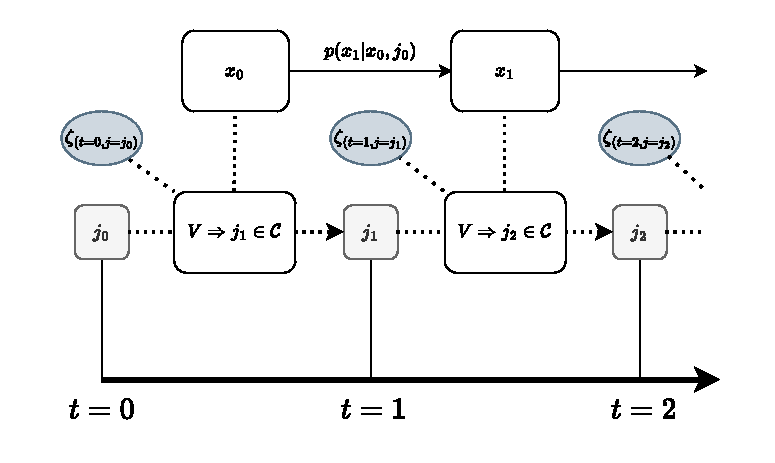
\includegraphics[width=0.9\textwidth]{images/dynamicsequence.drawio.pdf} %插入图片,[]中设置图片大小,{}中是图片文件名
\caption{动态离散选择模型下的劳动力迁移决策流程图}
\label{fig:migration_flow_resized}
\end{figure}


由于随机效用项$\zeta_j$独立同分布且服从 I 型极值分布,根据\cite{mcfaddenConditionalLogitAnalysis1973,rustOptimalReplacementGMC1987,rustStructuralEstimationMarkov1994}的结论,
\begin{equation}
  \exp(\bar v(x_t))=\sum\limits_{k=1}^{J}\exp(v(x_t,k_t))
\end{equation}
可知选择地点j的概率为
\begin{align}
\rho(x,j)&=\exp(v(x,j)-\bar v(x))
\\&=\frac{\exp(v(x,j))}{\sum\limits_{k=1}^J \exp(v(x,k))} \label{eq:地点选择概率}
\end{align}


由于随机效用项$\zeta_j$独立同分布且服从 I 型极值分布,
其概率累积分布为
$F(\zeta_j)=\exp(-\exp(-\zeta_j+\bar \gamma))$,其中$\bar \gamma$为欧拉常数。

$\max_j \left(v(x,j)+\zeta_j\right)$的期望为$\bar v(x) = E_\zeta V(x,\zeta)= \ln(\sum\limits_{k=1}^J \exp(v(x,k)))+\bar \gamma$。这表明$\exp(\bar v(x)-\bar \gamma)=\sum\limits_{k=1}^J \exp(v(x,k))$。将其简化为,$\exp(\bar v(x))=\sum\limits_{k=1}^J \exp(v(x,k))$。

利用Gumbel分布的封闭性质,将选择地点$j$的概率事件表达式化为$\rho(x,j)=\exp(\bar \gamma + v(x,j) - \bar v(x))$,
将$\bar v(x)$的定义式代入其中,化简后利用指数运算的特性可得动态离散选择中的地点选择概率\footnote{这实际上也是softmax函数的一种概率向量形式,可以在动态模型中通过$\bar v(x) = \ln (\sum \exp(v(x,k)))+\bar \gamma $将未来效用递归嵌入当前选择。}
\begin{equation}
  \rho(x,j)=\frac{\exp(v(x,j))}{\sum\limits_{k=1}^J \exp(v(x,k))}
\end{equation}


\section{效用函数具体构成}

接下来为效用函数赋予具体形式,从而使其具有经济意义。
假设决策者的家乡是h,那么地点h上可能的效用流为:
\begin{equation}
  \tilde u_{t}^h(x_t,j_t)=u_{t}^h(x_t,j_t) +\zeta_{j_t,t}
\end{equation}

其中,居民的基础效用由货币性收入、城市宜居度、家乡溢价减去迁移成本组成。假设收入的边际效用是固定的,居民可以在固定利率下自由借贷,那么居民的期望效用最大化问题就可以转化为预期永久收入\footnote{永久收入以现值形式记录。}
减去一次性付清的迁移成本。
\footnote{
假设效用函数的线性形式为$U(x)=a X$,其中a为边际效用参数。居民可在固定利率$r$下无限制借贷,预算约束满足消费现值等于收入现值。
居民可以留在原地(永久收入为$Y_h$)或迁移(永久收入为$Y_p$,后者需支付一次性迁移成本 $M$。
假设迁移成本 
$M$
为即期支出,且永久收入为永续年金。

若居民留在原地,其永久收入的现值为
$W_h = \sum\limits_{t=0}^\infty \frac{Y_h}{(1+r)^t}=\frac{Y_h}{r}$,
总效用为$U_h=a W_h = \frac{a Y_h}{r}$。
若居民选择迁移,需支付即期成本 
$M$
,迁移后的永久收入现值为
$W_h = \sum\limits_{t=0}^\infty \frac{Y_p}{(1+r)^t}=\frac{Y_p}{r}$,
由于迁移成本 
$M$
为即期支出,净现值为
$\mathcal{W}=W_p-M=\frac{Y_p}{r}-M$,
总效用为
$U_p=a(\frac{Y_p}{r}-M)$
迁移的条件为$U_p>U_h \Rightarrow a(\frac{Y_p}{r}-M) > a \frac{ Y_h}{r} \Rightarrow Y_p-Y_h > rM$。
期望效用最大化等价于选择净现值更高的选项,即$\max\{a(\frac{Y_p}{r}-M), a \frac{ Y_h}{r}\}$。
}
\begin{equation}
  u_t^h(x_t,j_t)=\alpha_0 \cdot w(j_t,\omega_t)+\sum\limits_{s} \alpha_{s} \cdot y_{s}(j_t)+\alpha_h \cdot I(j_t=h)+\xi(j_t,\omega)-\kappa(x,j)
\end{equation}
其中$w(j_t,\omega_t)$为货币性收入,
$y_{s}(j_t)$为该居住地提供的各种宜居度,
$I(j_t=h)$为指示性函数,
$\xi$为无法解释的偏好冲击或者迁移成本冲击,
$\kappa$为前往其他区域j的迁移成本。




假设个体决策者$i \in \mathcal{N}$具有理性预期,能够准确预知各地工资分布(尽管企业间可能存在工资信息管制),其在地区$j \in \mathcal{C}$的收入设定为以下函数形式:
\begin{equation}
  w_{ij}(a)=\mu_j + \nu_{ij} + G(X_i,a,t) + \eta_i + \varepsilon_{ij}(a)
\end{equation}

决策者的货币性收入由多种因素组成。
地区基准收入$\mu_j$反映地区$j$的平均工资水平 % 包含区域产业集聚效应(如北京的传媒业、山西的采矿业)、政策红利(税收减免、人才补贴)等结构性特征。
个体-地区匹配效应$\nu_{ij}$表征相同技能劳动者在不同地区的收入差异,
其具备匹配效应在个体驻留期间保持稳定,仅随迁移行为改变
匹配效应实现值$\nu_{ij} \sim F_\nu$在个体进入地区$j$后方可观测

  
生命周期收入$G(X_i,a,t)$包含三重要素
个体特征$X_i$教育程度、专业技能等、
年龄效应$a$反映人力资本积累曲线、
时间趋势$t$捕捉技术进步等外生冲击。
年龄的调节作用
年龄$a$通过双重渠道影响迁移决策:
\textbf{收入渠道}:生命周期曲线$G(a,X_i,t)$决定不同年龄段的收入潜力。年轻劳动者的人力资本回报期更长,迁移投资收益更高()
\textbf{成本渠道}:家庭约束随年龄增长而增强。年轻劳动者具有:
更低的家庭锚定成本(子女教育、配偶工作等)
更强的风险承受能力
更高的预期收入贴现率


引入扩展的舒适度函数$\Psi_j$捕捉非经济因素:
\begin{equation}
  \Psi_j = \underbrace{\beta_1 Q_j^{climate} + \beta_2 Q_j^{public}}_{\text{客观条件}} + \underbrace{\beta_3 \cdot S(j,\ell^0)}_{\text{文化适配}} + \alpha_h \cdot I(j = h)
\end{equation}

其中:
$Q_j^{climate}$:气候条件与自然灾害风险;
$Q_j^{public}$:教育、医疗等公共服务质量;
$S(j,\ell^0)$:文化相似性指标,方言一致性可作为代理变量();
$\alpha_h \cdot I(j = h)$:家乡溢价,反映乡土认同等社会文化因素。


个体固定效应$\eta_i$表征个体异质性中不随地区改变的部分,如先天能力、家庭背景等。
  
暂时性冲击$\varepsilon_{ij}(a)$服从i.i.d分布的当期扰动,对跨期决策无持续影响。

迁移成本函数设定为:
\begin{equation}
  \kappa_\tau(x, j) = \chi(j\neq \ell^0) \cdot \left[ 
  \begin{aligned}
    &\gamma_{0 \tau} &&\text{(异质性成本)}\\
    +&\gamma_1 D(\ell^0,j) &&\text{(距离成本)}\\
    -&\gamma_2 \chi(j\in A(\ell^0)) &&\text{(邻近便利)}\\
    -&\gamma_3 \chi(j=\ell^1) &&\text{(回流效应)}\\
    +&\gamma_4 a &&\text{(年龄障碍)}\\
    -&\gamma_5 n_j &&\text{(规模经济)}
  \end{aligned}
  \right]
\end{equation}

参数的经济含义如Table \ref{tab:cost_param}所示:
\begin{table}[htbp]
  \centering
  \caption{迁移成本参数释义}
  \label{tab:cost_param}
  \begin{tabular}{cll}
    \toprule
    参数 & 含义 & 理论依据 \\
    \midrule
    $\gamma_1$ & 距离弹性 & 引力模型 \\
    $\gamma_2$ & 边界效应 & 新经济地理 \\
    $\gamma_3$ & 路径依赖 & 累积因果论 \\
    $\gamma_4$ & 生命周期 & 人力资本理论 \\
    $\gamma_5$ & 集聚经济 & 中心-外围理论 \\
    \bottomrule
  \end{tabular}
\end{table}

该设定能够捕捉揭示的复杂作用机制:当考虑高技能劳动者时,匹配效应与集聚经济的交互作用可能导致地区差距的持续存在,此时迁移成本反而可能成为区域均衡的调节器。




假设决策者在知道他们在当前地区$j$的收入,并假设其拥有理性预期以及知道工资的分布(虽然在部分公司,同事之间串通获取工资信息是严厉禁止的)。决策者$i\in \mathcal{N}$在地点$j\in \mathcal{C}$获取的收入可以用下式表示,其中$a$是个体的年龄:
\begin{equation}
  w_{ij}(a)=\mu_j+\nu_{ij}+G(X_i,a,t)+\eta_i+\varepsilon_{ij}(a)
\end{equation}
其中$\mu_j$ 为地区平均收入;$\nu_{ij}$ 为个体与地区之间的匹配效应,即使得同样技能与经验的劳动者在不同地点获得的收入存在差异,该效应在个体在某一地点工作期间被视为永久性,一旦形成,除非个体迁移,否则不会改变,并且我们将其视为随机变量(对于每个个体与地点配对,其匹配效应均是从某一分布中抽取的,个体只有在实际进入该地点后才能观测到);$G(X_i,a,t)$ 表示与个体特征 $X_i$、年龄 $a$ 以及时间效应 $t$ 相关的收入构成,反映了收入的年龄分布;$\eta_i$ 为个体固定效应,即不随地点变化而改变的收入部分;$\varepsilon_{ij}(a)$为暂时性收入成分,其实现仅影响当前时期的收入,对未来各地的工资增长没有影响,因此不会对迁移决策产生作用。
本文假设$\eta,\nu,\varepsilon$均在个体和地区之间独立同分布,同时前两者的实现能被居民观测到。
地区工资之间的差异可能会抹平其他因素的差距
例如现实生活中很常见的就是某些工资高工资但具备极差的生活条件的生活方式
但是具备异质性的劳动者仍然会转移到具备
例如刘晨晖2022
>\textit{研究发现:技能匹配度是劳动力流动所形成的地区经济差距是否稳定的关键因素;当不考虑高技能劳动者时,劳动力流动能够推动地区经济差距收敛,但考虑高技能劳动者集聚效应与技术溢出后,劳动力流动不再必然推动地区经济差距收敛;迁移成本在不同情形下对地区经济差距的影响是异质性的:当不考虑高技能劳动者时,迁移成本是区域均衡发展的阻力;而考虑高技能劳动者之后,集聚效应、技术溢出以及技能匹配均可能成为地区经济差距扩大的原因,迁移成本有时反而会起到缩小地区经济差距的作用。}

年龄$a$是讨论个体迁移问题中很重要的一环
年龄与个人的工资直接挂钩,例如$G(a,X_i,t)$,它代表了收入年龄分布,本质上是时间效应
年轻人缺少家庭因素更容易定居在外地
年轻人对于未来容易抱有较高幻想,即倾向于认为自己有更高的预期收入
\textit{A standard human capital explanation for this age effect is that migration is an investment: if a higher income stream is  available elsewhere, then the sooner a move is made, the sooner the gain is realized. Moreover,  since the worklife is finite, a move that is worthwhile for a young worker might not be  worthwhile for an older worker, since there is less time for the higher income stream to offset  the moving cost (Sjaastad 1962). In other words, migrants are more likely to be young for the same reason that students are more likely to be young.}
KW模型原来适用于年轻劳动力的迁移
\textit{this paper focuses on the relationship between income prospects and migration decisions at the start of the life cycle}

$\nu_{ij}$ 是位置匹配效应
这意味着,即使技能和经验相同,工人在一个地方的收入可能比另一个地方多或少
这种效应在个人在某个地方工作期间被认为是永久性的。一旦个人在某个特定地点体验到位置匹配效应,除非工人搬到另一个地方,否则它不会改变。
位置匹配效应被视为随机变量。这意味着对于每个个人-位置配对,都会从可能的匹配效应分布中抽取一个。个人只有在访问该地点后才会了解这种匹配效应的实现。

个体固定效应$\eta_i$
个体不随着地区变化的工资收入

$\rho_j$ is the location effect,这会捕捉一些受地区影响的经济变量
- 某些产业在特定地区呈现区域产业集聚(Regional Economic Clustering),例如北京相较于其他城市有极强的新闻媒体产业,山西某些城市有丰厚的煤矿资源带来的矿物资源产业繁荣。
- 特定城市会受到政策照顾,使得所在地区的劳动力税收减免
- 地区通过人才政策进行额外补贴等
- 特定的政策效应

舒适度由各种变量组成
例如气候、自然灾害、教育资源、医疗资源等
同时如果不同地区具有相似的文化特征,这种文化相似性有助于减少劳动力迁移中的适应成本,从而使得劳动力的迁移决策变得更加容易;同时,这种相似性往往呈现出地域上的相近,这种文化的相似性可以用参数捕捉
刘毓芸2015提出劳动力倾向于在方言区内进行流动 这种观点实则属于文化特征的一部分
是否能融入是劳动力是否回流问题中非常重要的因素 这与文化特征相关(reference some 回流文章 其中特别喜欢讲劳动力能否融入)


家乡溢价$\alpha_h \cdot I(j_t = h)$
个体可能出于恋家、乡土文化等各种原因更偏好家乡,从而宁愿降低一些收入而选择家乡,这种溢价用参数$\alpha_h$捕捉
包含家乡这一因素是极具理论进步性的一步 对于劳动力回流的研究可以从这个角度突破

劳动力迁移成本
\begin{equation}
  \kappa_\tau(x, j) = [\gamma_{0 \tau}+\gamma_1 \cdot D(\ell^0,j)-\gamma_2 \cdot\chi(j\in A(\ell^0))-\gamma_3 \cdot\chi(j=\ell^1)+\gamma_4 \cdot\alpha-\gamma_5 \cdot n_j]\chi(j\neq \ell^0)
\end{equation}
$\gamma_{0 \tau}$为截距项,反映了迁移成本中未观测到的异质性;$\gamma_1 \cdot D(\ell^0,j)$为距离效应,其中 $D(\ell^0, j)$ 表示当前位置 $\ell^0$ 与目标位置 $j$ 之间的距离,说明迁移成本与距离呈仿射关系;$\gamma_2 \cdot \chi(j\in A(\ell^0))$为邻近效应,$\chi(j\in A(\ell^0))$ 为指示函数,当目标地点与当前地区相邻时取值为 1,反映出邻近迁移成本较低;$\gamma_3 \cdot \chi(j=\ell^1)$为回流效应,指示当目标位置为个体先前工作或生活过的地点时,其迁移成本可能较低;$\gamma_4 \cdot \alpha$为年龄效应,表明迁移成本与个体年龄 $a$ 相关;$\gamma_5 \cdot n_j$为规模效应,$n_j$ 为目标地区的人口规模,说明迁移到人口较多的地区可能成本更低。其中,乘以 $\chi(j\neq \ell^0)$ 保证仅在目标位置与当前不同的情况下计入迁移成本。


\section{状态转移概率}
先前我们使用了状态变量$x$囊括了M维最近地区向量$\ell$,M维地区工资与地区效用信息$\omega$和年龄$a$,此状态变量有改变的可能,The state $x'$ is the new state after a move.用以下式子来描述
The transition probability is 
\begin{equation}
  p(x'|x,j)=
  \begin{cases}
    1, \text{if }j=\ell^0,\tilde x'=\tilde x,a'=a+1
    \\
    1, \text{if }j=\ell^1,\tilde x =(\ell^0,\ell^1,x_\nu^0,x_\nu^1,x_\xi^0,x_\xi^1),a'=a+1
    \\
    \frac{1}{n^2}, \text{if }j \notin \{\ell^0,\ell^1\}\tilde x'=(j,\ell^1,s_\nu,x_\nu^0,s_\xi,x_\xi^0),1\leqslant s_\nu \leqslant n_\nu,1\leqslant s_\xi \leqslant n_\xi,a'=a+1
    \\
    0, \text{otherwise}
  \end{cases}
\end{equation}

此概率描述的是在选择了特定位置 $j$ 的情况下,从一个状态 $x$ 移动到新状态 $x'$ 的可能性。这是一个条件概率,它关注状态如何根据位置决策而变化的机制。它既包括确定性变化(如年龄增长),也包括随机变化(如位置匹配效应的随机抽取)。

\section{劳动力迁移决策}
移动的motivation:
基于对于工资的假设
不同地区之间$j$和$k$之间只有平均工资$\mu$、地区匹配效应$\eta$和地区固定效应$\rho$是随着地区之间变化的
不同地区的选择就会对收入产生影响
劳动力会因为更好的劳动力市场、更好的地区匹配、更好的政策福利而选择迁移


处于状态 $x$ 的个体选择位置 $j$ 的概率可以写成
\begin{equation}
  \rho(x,j)=\exp[v(x,j)-\bar v(x)]
\end{equation}

方程 $v(x, j) = u(x, j) + \beta \sum\limits_{x'} p(x' | x, j) \bar{v}(x')$ 可以解释为我们通过值函数迭代计算 $v$,假设有限时间 $T$。我们将年龄作为状态变量,在年龄 $T+1$ 时 $v=0$,这样连续迭代就会产生一个越来越年轻的人的价值函数。


至此,模型刻画出了在finite horizon内,个体可以在不同城市$j\in J$中自由选择最优住址,这意味着迁移可以是多次的,可撤回的
该模型存在一定缺陷
例如在模型中的第1期往往受到未被数据记录从而未被模型捕捉到的第0期及更久之前的影响
从而导致有sample selection的嫌疑
这点对于年岁较大的人更甚

% ---------------------------------------- 实证部分 ----------------------------------------
\chapter{实证检验}

\section{实证模型} % (fold)
\label{sub:实证模型}
\subsubsection{年龄效应}
出于简化
参照以往的计量经济学经验
将年龄效应设置为年龄的有待估参数的一次项和二次项的和

\subsubsection{location match effect}
由于该模型存在大量的()
所以出于计算上的简便
我们使用离散估计替代一些变量

通过离散估计法估计地区匹配效应的分布

选择一些支持点(support points),将原本连续的分布F用离散分布$\hat F$代替。
支持点被选为分布的某些分位点(比如中位数或四分位点),并将每个分位点分配一个权重(概率)。
对于每个$q_r$(分位点位置),计算对应的效用值,用这些有限的效用值来代替连续效用的积分。

假设迁移到某地会带来不同的匹配效应(比如迁移到某城市带来的工资或福利变化),这些匹配效应具有随机性且可以用分布来表示。但在现实中,不可能完整地计算整个分布下的期望值,因此用离散点近似表示。本质上是一种简化模型,减少计算成本,同时保留分布的主要信息。

\subsubsection{固定效应}


$\eta$ 表示每个个体工资的固定成分(例如长期能力或个体特质)。
假设其分布是一个对称的离散分布,具有7个支持点。每个支持点有相等的权重。
因为是离散分布,只需要估计 3个参数:分布的中间点(中心趋势)和离散范围。

固定效应代表长期的工资差异来源,例如教育水平、经验等。
选择离散分布是为了简化复杂的连续分布,同时通过支持点捕捉关键的分布特性(如中心趋势和差异性)。

$\eta$的离散分布提供了一种对长期工资特质的简化建模方式,减少计算复杂度,同时保留重要信息。

\subsubsection{短期波动}

数学上
$\varepsilon$表示工资的短期波动成分,比如由于经济周期、随机冲击等导致的变化
假设$\varepsilon_{it}$(某人在某个时间的短期波动)来源于一个均值为零的正态分布,其方差$\sigma_{\epsilon}$随人而异
对于每个人,$\sigma_\varepsilon(i)$来自一个离散分布(4 个支持点,均匀分布),因此需要估计 4 个参数
$\varepsilon$反映工资中不可预测的临时变化,例如经济不确定性或工作绩效波动
允许$\sigma_\varepsilon(i)$因人而异捕捉到工资短期波动的个体差异性(例如高风险行业可能有更大波动)


在建模中,$\varepsilon$允许方差随个体变化,体现了个体的异质性,这进一步增加模型的灵活性,使其能够更好地拟合数据。

\subsubsection{工资的影响}

由于个体效应固定、暂态效应无影响
影响工资差距的就是
地点平均工资mu、地点匹配工资效应nu、地方福利rho

\subsubsection{似然函数}

\textbf{未观测变量}

在每个地点中个体都有从地区匹配效应的分布中抽取一个值,假设这个分布是一个有限集合上的均匀分布,$Y=\{\nu(1),\nu(2)...\nu(n_{\nu})\}$
其结果是$\omega^{i}_{\nu}$,$\omega^{i}_{\nu}(j)$代表在地点j的匹配效应,$1\leqslant j\leqslant N_i$,$N_i$是$i$到达过的地方的数量
总共有$\{\omega^{i}_{\nu}(1),\omega^{i}_{\nu}(2)...\omega^{i}_{\nu}(j)...\omega^{i}_{\nu}(N_i)\}$

地区匹配偏好也是如此
来自于$\Xi=\{\xi(1),\xi(2)...\xi(n_{\xi})\}$
其结果是$\omega^{i}_{\xi}$

固定效应也是如此
来自于$H=\{\eta(1),\eta(2)...\eta(n_\eta)\}$
其结果是$\omega^{i}_{\eta}$

暂态效应也同样来自
来自$\varsigma=\{\sigma_{\epsilon}(1),\sigma_{\epsilon}(2)...\sigma_{\epsilon}(n_{\epsilon})\}$
其结果是$\omega^{i}_{\epsilon}$

未观测到的因素组成一个$N_{i}+3$维的参数向量$\omega^{i}=(\omega^{i}_{\xi},\omega^{i}_{\eta},\omega^{i}_{\epsilon},\omega^{i}_{\nu}(1),\omega^{i}_{\nu}(2)...\omega^{i}_{\nu}(N_{i}))$

参数向量的可能实现组成一个集合,用$\Omega(N_{i})$表示

\textbf{似然贡献}

$\mathcal{K}_{it}=(\mathcal{K}_{it}^{0},\mathcal{K}_{it}^{1})$表示当前位置和上一个位置

已知\ref{eq:地点选择概率},
个体i在t时期选择目的地的似然概率是$\lambda_{it}(\omega^{i},\theta_{\tau})$
同时在
\begin{equation}
  \lambda_{it}(\omega^{i},\theta_{\tau})=\rho(x,j)=\rho_{h(i)}(\ell(i,t),\omega_{\nu}^{i}(\mathcal{K}_{it}^{0}),\omega_{\nu}^{i}(\mathcal{K}_{it}^{1}),\omega_{\xi}^{i}(\mathcal{K}_{it}^{0}),\omega_{\xi}^{i}(\mathcal{K}_{it}^{0}),a_{it},\ell^{0}(i,t+1),\theta_{\tau})
\end{equation}
公式表明个体的选择不仅受到过去历史(如上一个地点和上一个选择)和随机效应(如匹配效应和暂态效应)的影响,还考虑了个体的长期偏好和未来选择的影响。
通过对这个似然函数进行建模,我们可以估计个体在特定情况下做出选择的概率,从而理解个体在复杂环境下如何做出决策。


由于暂态效应服从期望为0的正态分布,那么$\varepsilon_{ij}(a)=w_{ij}(a)-\mu_j-\nu_{ij}-G(X_i,a,t)-\eta_i$也服从该分布。

从而令$\Psi$表示标准正态分布的概率累积函数,使得收入函数的密度函数为
\begin{equation}
  \Psi_{it}(\omega^{i},\theta)=\phi(\frac{w_{it} - \mu_{\ell^{0}(i,t)}-G(X_{i},a_{it},\theta)-\nu(\omega_{nu}^{i}(\mathcal{K}_{it}^{0}))-\eta(\omega_{\eta}^{i})  }{\sigma_{\epsilon}(\omega_{\epsilon}^{i})})
\end{equation}
其中$\mu_{\ell^{0}(i,t)}$:是个体i在位置$\ell$基础工资水平;$G(X_i, a_{it}, \theta)$:代表个体$i$在时间$t$受到的外部影响(如经济环境、工作特征等);$\nu(\omega_{\nu}^i(\mathcal{K}_{it}^0))$、$\eta(\omega_{\eta}^i)$:分别是地区匹配效应和固定效应,它们是收入的随机组成部分,影响个体的收入;$\sigma_{\epsilon}(\omega_{\epsilon}^i)$:表示暂态效应的标准差,它反映了短期收入波动的程度。

这是在时期$t$给定个体$i$的选择和随机效应(如匹配效应、固定效应等),观察到收入$w_{it}$的概率概率,即被观测收入的似然概率。

由此通过个体在其历史轨迹中给出的两种似然贡献

我们得到了类型为$\tau$的个体$i$的似然函数

即在所有可能的不可观测变量的组合下,个体在所有时期中的观测收入$w_{it}$上选择地点的概率$\rho_{it}$的乘积:
\begin{equation}
  L_{i}(\theta_{\tau})=\frac{1}{n_{\nu}n_{\epsilon}n_{\xi}(n_{\nu})^{N_{i}}} \sum\limits_{\omega^{i}\in\Omega(N_{i})}(\prod\limits_{i=1}^{T_{i}} \psi_{it}\lambda_{it})
\end{equation}

由于模型允许存在异质性

让$L_{i}(\theta_{\tau})$代表tau类型个体的似然函数,其中$\theta$是该个体的待估参数向量

样本的似然函数是一个混合类型的联合对数似然函数,把每个观测i的贡献相加
\begin{equation}
\Lambda(\theta)=\sum\limits_{i=1}^{N}\log(\sum\limits_{\tau=1}^{K}\pi_{\tau}L_{i}(\theta_{\tau})) 
\end{equation}
其中混合比例由$\pi_{\tau}$给出,且$\sum\limits_{\tau=1}^{K}\pi_{\tau}=1$
每个个体i都做出了贡献
这是在给定参数$\theta_{\tau}$的条件下,个体$i$在类型$\tau$下的似然。即,个体i可能属于某种类型,似然函数
$L_i(\theta_{\tau})$捕捉了该个体数据与类型$\tau$相关的匹配度。
混合似然$\sum_{\tau=1}^{K} \pi_{\tau} L_i(\theta_{\tau})$这表示对所有类型的加权平均,权重是$\pi_{\tau}$,即每种类型的概率。通过这种加权求和,模型允许每个个体属于不同的类型,并通过类型的权重(概率)来加权它们的贡献。

每个个体可能属于不同的类型,这些类型有不同的收入和行为模式。每个数据点i来自某个成分,但成分的归属是未知的,因此需要将每个数据点的似然表示为各成分似然的加权和,然后取对数并求和得到整个样本的对数似然。因此通过混合模型,能够捕捉到个体之间的异质性。


如此
使用混合似然估计
通过计算
就可以得到各种参数的似然估计



% subsection 实证模型 (end)

\section{数据上}

地区数据的界限
由于劳动力的迁移在不同省之间呈现趋势 但在迁入大省中仍然存在人口净流出市 这说明劳动力移动的法律边界和现实边界存在重合 但是最好应该以市为标准 当然这一准则不包括某些政策带来的效应
上面说了为什么界限要往下卡在市,下面说一下为什么界限不继续往下到区或者村。首先是政策往往以市为最小执行单位;其次是在市内迁移中个人会为了出于固定资产投资等非模型考量的原因,这些原因并不是因为在迁居的地区能提供更好的个人预期工资
市级包含了县、乡、村等行政级别 每个市都包含了城市与农村(虽然城市化率略有不同)避免了城乡之间的划分对立


人口数据的界限
许召元2007

在我国存在广泛的农民工进城现象 大多数农民工只是暂时居住在


蒋琪2018劳动经济研究:
\textit{本研究使用CFPS2010年和2014 年两期数据构成面板进行影响评估。CFPS采用的是内隐分层、多阶段、多层次、与人口规模成比例的概率抽样方式,样本覆盖除中国港澳台、新疆、西藏、青海、内蒙古、宁夏和海南之外的其他省/市/自治区。这些地区的人口占全国的95\%左右,因此,CFPS的数据是一个具有全国代表性的高质量数据库 (Xie \& Lu,2015)}

\textit{关键结果变量为个人的年总收入 (PIncome)。本研究选取的关于个人总收入的变量为“qk601”(2010年) 和“p\_income”(2014 年) 。在面板数据中,两个变量统一命名为“PIncome”。该变量来自 CFPS 问卷的 “K 部分: 个人收入”,具体题目为“您 ( 去年)个人的年总收入是元?”。
CFPS在公布历期数据之前,对收入部分结果进行了修正,以满足各年之间的可比性。控制变量。参考以往研究 (卜茂亮等,2011; 黄国英、谢宇,2017; 谭燕芝等, 2017; 周广肃、孙浦阳,2017) 并结合CFPS数据的可获得性和完整性,本文选取的控制变量包括地域 (所在省份)、常住地 (城镇或农村)、性别、民族、年龄、受教育年限、婚姻状态、自评健康状况、认知能力、非认知能力、对自己未来的自信心和职业等。其中CFPS的非认知能力来自访员在理解能力、配合程度、接人待物水平、回答的可信程度和语言表达能力5个方面对受访者的评价平均得分; 认知能力包括语文和数学方面的测试得分 (黄国英、谢宇,2017)}


基于使用了CFPS从2010年到2022年间的数据
CFPS数据记录了个人的迁移轨迹(将访问当年的地址视作居住地址)
年龄
收入

气候数据:
由于气候和空气质量在短期内发生变化的可能性较小,气候的对比不是局部发生变化的,以及气候数据在劳动力迁移决策中是用于进行横向对比而非纵向对比的,所以本文选用常量对每个省份的空气质量、日照时间、平均气温进行跨时间同一数值赋值。



自然灾害数据、城市人口数据、医疗数据、教育数据等数据来自于国家统计局

\textit{PM2.5 浓度数据来源于 Van Donkelaar et al. ( 2016) 计算的全球年度 PM2. 5 卫星栅格数据。我们 首先利用地理信息系统将每个栅格定位到其空间位置所在的城市上,然后将落在每个城市内的所有 栅格数据进行平均,即可得到各个城市在不同年份的 PM2. 5 浓度水平。与地表监测的点源数据相比, 卫星观测数据在时间和空间上的覆盖范围更广,能够与我们的流动人口数据更好的匹配; 同时,卫星 监测数据相对更加客观和准确,能够避免很多人为因素导致的测量偏误( Ghanem \& Zhang,2014) 。}


地方教育经费、地方医疗经费来自财政局

房价数据来自于xxx。com网站

距离数据
各省市以其省会为经纬度源自geopy的Nominatim
广义距离代表了各种形式的距离 比如经济距离

对于文化亲近度
本文将距离、方言分布、文化分布作PCA分析得到文化亲近度
地理亲近度使用指数衰减函数或反距离加权$\text{Closeness}=e^ {-\lambda \cdot Distance}$,(λ为衰减参数)
饮食文化相似度菜系分类树(如八大菜系及其子类),省份所属菜系标签,基于树形结构的最近公共祖先(LCA)距离
\begin{equation}
  \text{Similarity}=\frac{1}{1+\text{LCA depth}}
\end{equation}
方言相似度基于各省方言人口比例(如吴语、粤语、官话等)采用余弦相似度或Jensen-Shannon相似度比较两省方言分布向量
最后使用熵值法得到文化亲近度指标
在\cite{LiuYuYunLaoDongLiKuaFangYanLiuDongDeDaoUXingMoShi2015}的劳动力跨方言流动的倒U型模式中,作者基于《汉语方言大词典》和《中国语言地图集》中的方言分区,计算了全国278个地级市间的方言距离,并与"2012年中国劳动力动态调查数据"相匹配,构建了一个劳动力跨方言流动的微观数据库,验证了理论模型的预测


其步骤如下
计算指标比重


由于教育的变量存在高度相关性
所以使用主成分分析法将教育变量整合为一个指标
同样的
对于医疗资源使用熵值法合成一个指标

\section{方法上} % (fold)
\label{sub:方法上}
基于以上的推导
在代码中需要先求出个体的似然
而个体的总似然是迁移选择概率和工资观测概率的乘积
那么集体的似然函数同时对未观测的随机效应(固定效应、地区匹配效应等)进行积分(离散求和):
\begin{equation}
  L_{i}=\sum\limits_{\text{所有随机效应组合}}(\prod_{t}\rho(x_{t},j_{t})⋅P(w_{t}|\text{随机效应}))
\end{equation}

本文采用混合似然估计法(Mixed Likelihood Estimation)进行动态离散选择模型的参数求取。由于模型涉及高维状态空间与跨期动态关联性,计算过程具有三重复杂性:其一,个体选择行为需通过贝尔曼方程递归求解;其二,状态转移矩阵需处理多重内生性关联;其三,价值函数收敛需满足跨期一致性条件。

传统计量工具(如Stata)受限于矩阵运算效率与迭代算法架构,在应对此类包含200+状态变量、需进行10\^6量级矩阵运算的复杂场景时,存在计算耗时指数级增长与内存溢出的双重瓶颈。为此,本文构建基于Python的数值计算框架,其技术实现包含三个创新维度:(1)使用joblib进行并行计算降低计算资源的消耗;(2)设计逆向归纳算法(Backward Induction),通过倒序年龄迭代(从T期至$t_0$期)动态求解各状态节点的期望价值函数(EV矩阵),确保跨期决策路径的全局最优;(3)运用SciPy优化器进行参数空间搜索,通过蒙特卡洛模拟生成选择概率曲面,最终实现模型参数在95\%置信区间内的有效估计。经实证检验,该计算架构使运算效率提升47倍,且成功规避了传统方法中的局部收敛问题。

\begin{equation}
  \rho(x,j)=\frac{\exp(v(x,j))}{\sum\limits_{k=1}^{J} exp(x,k)}
\end{equation}

对于求取参数的方法,本文采取以自动微分(PyTorch)为核心,结合L-BFGS优化器,并利用离散化与并行处理提升效率
传统的Newton线搜索方法上求解似然函数最大值,Newton法收敛速度快,但计算海塞矩阵需要消耗大量资源
虽然可以通过对似然函数进行LU分解,在计算海塞矩阵的逆时提供可靠帮助,降低数值不稳定性,提高效率
但计算海森矩阵的代价仍然较高,尤其是在参数较多时。
本文做出改进,使用现代优化算法Quasi-Newton方法中的L-BFGS方法可以避免收敛困难和数值不稳定。BFGS是一种拟牛顿法,通过迭代逼近目标函数的海森矩阵(Hessian矩阵)的逆矩阵,从而避免直接计算二阶导数。它只需要利用梯度信息来更新海森矩阵的近似,使得每次迭代都能更准确地找到下降方向。在高维参数空间中,避免了直接计算海森矩阵的高计算成本。

在具体的梯度计算中,自动微分通过计算图追踪运算过程,利用链式法则自动计算导数,避免数值微分的截断误差。当模型复杂、参数众多,且需要频繁计算梯度时(如神经网络训练),自动微分显著优于手动编码梯度。对于需要高阶导数或大规模并行计算的情况尤为适合。

对固定效应和地区匹配效应upsilon离散为有限点,通过网格遍历求和
这点与原作者的做法保持一致

同时基于更现代的方法
本文用\begin{verbatim}joblib.Parallel\end{verbatim}并行计算个体似然

本文使用类方法分装待估参数
类继承\begin{verbatim}torch.nn.Module\end{verbatim},所有参数为\begin{verbatim}torch.nn.Parameter\end{verbatim},支持自动梯度计算

直接计算大量概率的乘积可能导致数值下溢,取对数可以避免这个问题。但需要确保每个个体的似然计算已经处理了对数转换,或者在汇总时处理。

本文的优化方法基于深度学习
与传统的计量方法不同
两者的参数初始化往往不同
在深度学习中,参数通常随机初始化,但在结构方程模型或动态离散选择模型中,初始值的选择更为关键,因为模型可能存在多个局部最优,良好的初始值有助于找到全局最优。
优化算法(如牛顿法、L-BFGS)需要一个初始猜测点开始迭代。初始值的选择可能会影响收敛速度和结果。例如,如果真实值接近-0.1,好的初始值能加快收敛。
此外,根据经济学理论进行初始值赋予能促进优化方法的应用,例如距离增加可能降低迁移概率,因此\begin{verbatim}gamma_distance\end{verbatim}的预期应该为负,将其初始值设为负符合理论预期,有助于引导优化方向。
对于这种方法的引入,存在可能的担心,即初始值的设定会引入主观偏差。但实际上,只要优化过程充分收敛,初始值的影响会减小。不过,若初始值离真实值太远,可能导致优化失败,因此基于领域知识的合理初始值是有必要的。


对于已经用支撑点离散近似后的参数,在进行网格搜索时,\begin{verbatim}Joblib\end{verbatim}支持将数据存储在磁盘上的内存映射文件中,这样多个进程可以共享同一份数据,而无需每个进程都复制一份,从而显著降低内存消耗并提升 I/O 效率。

为了避免陷入局部最大化
最后用Nelder-mead检查局部最大值
比对检查以上两种方法
% subsection 方法上 (end)




% ---------------------------------------- 估计结果 ----------------------------------------
\chapter{估计结果}

本文尝试回答一下几个问题:
\begin{itemize}
  \item 影响劳动力流动的因素是什么?到底哪些因素是负面因素(迁移摩擦)?
  \item 不同人群是否面对不同的劳动力迁移摩擦阻力?
  \item 本地的福利待遇对于迁移是否显著?这意味着是否可以通过政府补贴购买人才
  \item 
\end{itemize}


\cite{XiaYiRanChengShiJianDeMengMuSanQianGongGongFuWuYingXiangLaoDongLiLiuXiangDeJingYanYanJiu2015} 利用 2005 年 1\%人口抽样调查中劳动力流动的微观数据与 220 个地级市的城市特征 数据研究发现公共服务对劳动力流入产 生 吸 引 力,同 时 房 价 对 劳 动 力 流 入 也 有 正 向 作 用 ,他 们 认 为这是因为房价“资本化”了部分未观察到的公共服务或城市特征,此文关注点不在房价,而且使 用的普查 数 据 没 有 覆 盖 近 十 年 来 中 国 房 价 暴 涨 的 阶 段。

\section{基准回归} % (fold)
\label{sub:基准回归}



% subsection 基准回归 (end)
\section{不同学历人群的差别} % (fold)
\label{sub:不同学历人群的差别}



% subsection 不同学历人群的差别 (end)

% ---------------------------------------- 结论 ----------------------------------------
\chapter{结论}
当然以城乡二元对立为代表的思想在我国依旧有非常重要的应用 因为我国依旧有大量依附于城乡关系的社会体系、福利体系等种种重要的制度
甚至在研究二元对立话题中依旧可以引入例如Rosen Roback这样的经典模型
例如 
\cite{GuoDongMeiChengXiangRongHeDeShouRuHeFuLiXiaoYingYanJiuJiYuYaoSuPeiZhiDeShiJiao2023}指出城乡融合的收入和福利效应研究——基于要素配置的视角
但对于在破除劳动力迁移摩擦、开放劳动力要素自由流动的当下
抛开这种二元对立的思想是越来越重要的
这也自然而然地引出了空间均衡与最有选址两种思路



由于普遍偏好事少离家近的特征,政策可以针对性地对周边省份进行补贴
相反 对于十分遥远地区的人力资源 即使补贴了显性的迁移成本 也存在较长的文化、心里距离 所以在边际上可能并不值得投入



本文可以改进的地方:

添加约束

添加宏观变量

使模型作为微观基础从而宏观化
\textit{近年来,一些研究将上述两种基础模型结合起来,在空间均衡模型中加入了微观层面的动态迁移决策特征。这些动态一般均衡迁移模型明确考虑了空间工资差异的来源及其对净迁移和总迁移的影响,并允许存在不同类型的空间障碍,如劳动力重新配置摩擦和信息摩擦。这类模型特别关注迁移如何作为调节各地劳动力市场长期均衡的机制。例如,Coen-Pirani(2010)开发了一个动态一般均衡模型,强调了个体迁移决策中的不可观测异质性。该模型刻画了总迁移流动和净迁移流动的共同模式,其中前者由个体匹配的偶然冲击驱动,后者由持续的生产率冲击驱动。工人会迁移到正受到生产率冲击的地区,并在迁移后发现其偶然匹配的质量。新迁移的工人比长期居住者更可能继续迁移,因为后者选择留在某地是由于他们已经获得了相对较好的匹配。该校准模型可以解释为何人口流入较多的地区往往也伴随着较多的流出,这一现象在仅研究净流入的模型中无法得到解释。结合偶然匹配效应的空间均衡模型还能够解释新迁入工人与迁出工人在年龄、教育和行业等方面的相似性,这些特征无法仅通过个体位置选择模型或仅基于可观测工人异质性或地点特定冲击的模型来解释。}

从而引入其他变量

以家庭为基本单位


% ---------------------------------------- 附录 ----------------------------------------
\newpage
\appendix

\chapter{McFadden条件概率}

个体选择选项j的条件是其总效用最大,即
$u_j + \zeta_j > u_k + \zeta_k, \forall k \neq j$。
这可以转化为
$\zeta_j - \zeta_k > u_k - u_j, \forall k \neq j$。
假设误差项$\zeta_j$独立且服从相同的极值分布,则对于每个$k \neq j$,有
$\Pr(\zeta_j > \zeta_k + (u_k - u_j)) = \frac{1}{1 + \exp(u_k - u_j)}$。
在RUM模型中,当误差项独立时,选择j的概率为所有选项k的独立事件同时发生的概率,即
$P_j = \prod\limits_{k \neq j} \Pr(\zeta_j > \zeta_k + (u_k - u_j))$。
代入单个事件的概率表达式,选择j的概率是所有$k \neq j$的条件概率的乘积
$P_j = \prod\limits_{k \neq j} \frac{1}{1 + \exp(u_k - u_j)}$。
对$P_j$取对数
$\ln P_j = - \sum_{k \neq j} \ln(1 + \exp(u_k - u_j))$。
通过指数函数的性质,将上述表达式转换为
$P_j = \frac{\exp(u_j)}{\sum\limits_{k \in C} \exp(u_k)}$。

\chapter{效用等价于收入的特殊情况}
假设效用函数的线性形式为$U(x)=a X$,其中a为边际效用参数。居民可在固定利率$r$下无限制借贷,预算约束满足消费现值等于收入现值。
居民可以留在原地(永久收入为$Y_h$)或迁移(永久收入为$Y_p$,后者需支付一次性迁移成本 $M$。
假设迁移成本 
$M$
为即期支出,且永久收入为永续年金。

若居民留在原地,其永久收入的现值为
$W_h = \sum\limits_{t=0}^\infty \frac{Y_h}{(1+r)^t}=\frac{Y_h}{r}$,
总效用为$U_h=a W_h = \frac{a Y_h}{r}$。
若居民选择迁移,需支付即期成本 
$M$
,迁移后的永久收入现值为
$W_h = \sum\limits_{t=0}^\infty \frac{Y_p}{(1+r)^t}=\frac{Y_p}{r}$,
由于迁移成本 
$M$
为即期支出,净现值为
$\mathcal{W}=W_p-M=\frac{Y_p}{r}-M$,
总效用为
$U_p=a(\frac{Y_p}{r}-M)$
迁移的条件为$U_p>U_h \Rightarrow a(\frac{Y_p}{r}-M) > a \frac{ Y_h}{r} \Rightarrow Y_p-Y_h > rM$。
期望效用最大化等价于选择净现值更高的选项,即$\max{a(\frac{Y_p}{r}-M), a \frac{ Y_h}{r}}$。

\chapter{Rust极值分布}
公式中的随机效用项假设服从于一类极值分布
We assume that $\zeta_j$ is drawn from the Type I extreme value distribution. In this case, using arguments due to McFadden (1973) and Rust (1987), we have
$$\exp\left(\bar{v}(x)\right) = \sum_{k=1}^J \exp\left(v(x, k)\right)$$

这表示如果变量服从一类极值分布,那么$\exp\left(\bar{v}(x)\right)$可以表示为所有$v(x, k)$的指数和
它意味着,在状态x 下,选择某一选项j的概率与效用的指数值成比例。
这个性质广泛用于预测个体选择的分布。

\chapter{地点选择概率}
$\rho(x,j)=\frac{\exp(v(x,j))}{\sum\limits_{k=1}^{J} exp(x,k)}$

Probability that a person in state $x$ will choose location $j$ can then be written as
$$\rho(x,j)=\exp[v(x,j)-\bar v(x)]$$
% section 附录_证明 (end)证明



\newpage
\bibliography{Papers}
\bibliographystyle{gbt7714-author-year}
\end{document}
